\documentclass[]{elsarticle} %review=doublespace preprint=single 5p=2 column
%%% Begin My package additions %%%%%%%%%%%%%%%%%%%
\usepackage[hyphens]{url}

  \journal{Global Environmental Change} % Sets Journal name


\usepackage{lineno} % add
  \linenumbers % turns line numbering on

\usepackage{graphicx}
%%%%%%%%%%%%%%%% end my additions to header

\usepackage[T1]{fontenc}
\usepackage{lmodern}
\usepackage{amssymb,amsmath}
\usepackage{ifxetex,ifluatex}
\usepackage{fixltx2e} % provides \textsubscript
% use upquote if available, for straight quotes in verbatim environments
\IfFileExists{upquote.sty}{\usepackage{upquote}}{}
\ifnum 0\ifxetex 1\fi\ifluatex 1\fi=0 % if pdftex
  \usepackage[utf8]{inputenc}
\else % if luatex or xelatex
  \usepackage{fontspec}
  \ifxetex
    \usepackage{xltxtra,xunicode}
  \fi
  \defaultfontfeatures{Mapping=tex-text,Scale=MatchLowercase}
  \newcommand{\euro}{€}
\fi
% use microtype if available
\IfFileExists{microtype.sty}{\usepackage{microtype}}{}
\bibliographystyle{elsarticle-harv}
\ifxetex
  \usepackage[setpagesize=false, % page size defined by xetex
              unicode=false, % unicode breaks when used with xetex
              xetex]{hyperref}
\else
  \usepackage[unicode=true]{hyperref}
\fi
\hypersetup{breaklinks=true,
            bookmarks=true,
            pdfauthor={},
            pdftitle={Mobility and flexibility enable resilience of human harvesters to environmental perturbation},
            colorlinks=false,
            urlcolor=blue,
            linkcolor=magenta,
            pdfborder={0 0 0}}
\urlstyle{same}  % don't use monospace font for urls

\setcounter{secnumdepth}{5}
% Pandoc toggle for numbering sections (defaults to be off)


% tightlist command for lists without linebreak
\providecommand{\tightlist}{%
  \setlength{\itemsep}{0pt}\setlength{\parskip}{0pt}}



\usepackage{graphicx}
\usepackage{booktabs}
\usepackage{tabularx}
\usepackage{multirow}
\usepackage{array}



\begin{document}


\begin{frontmatter}

  \title{Mobility and flexibility enable resilience of human harvesters to
environmental perturbation}
      
  \begin{abstract}
  Sustainable management of ecosystem services requires knowledge of both
  natural and human systems, but the adaptive behaviors of human
  harvesters in response to management changes and environmental
  variability are poorly understood. Given the specter of accelerating
  climate change, it is especially critical to understand how human
  harvesters may respond to environmental perturbation. In this study, we
  identify characteristics that promoted resilience of one the most
  valuable fisheries on the west coast of the United States to a record
  marine heatwave. Using movement telemetry linked to fishery landings
  records from more than 500 fishing vessels, encompassing 2.2 million
  geolocations and more than USD two billion in revenue, we found that
  vessels employed two, non-mutually exclusive strategies to cope with the
  anomalous environmental and management conditions imposed by the
  heatwave: increasing spatial mobility and diversifying fishery
  participation. The combination of these strategies appeared to be the
  most adaptive, as it produced the greatest increase in Dungeness crab
  profits. In contrast, participants that specialized in a single fishery
  and concentrated fishing effort in small spatial areas did not perform
  as well. Our data-driven approach reveals behaviors that can be promoted
  to improve the adaptive capacity of human harvesters in an era of
  unprecedented environmental perturbation.
  \end{abstract}
   \begin{keyword} climate change adaptation \textbar{} environmental perturbation
\textbar{} marine heatwave \textbar{} fisheries dynamics\end{keyword}
 \end{frontmatter}

\hypertarget{intro}{%
\section{Introduction}\label{intro}}

Sustainability in social-ecological systems---the continued provision of
human and ecological benefits from healthy ecosystems (Leslie et al.,
2015)---requires ecosystem and human resilience to environmental
perturbations. Just as species with similar ecological niches may react
differently to physical changes in their environments (Elmqvist et al.,
2003), human and ecosystem responses to perturbations can be diverse.
Resource users with diverse livelihood portfolios, available capital, or
distinct spatial patterns of resource extraction behavior do not respond
homogeneously to environmental or management changes (Young et al.,
2019). The behavior of human actors is further confounded by the
additional constraints associated with regulations and resource
management (Mcginnis and Ostrom, 2014). More conservative users might
rely on established knowledge and previously reliable spatial patterns
of exploitation, while others might adopt riskier, more exploratory
strategies that could lead to higher profits (Cohen et al., 2007).
Understanding the adaptive behaviors of resource users is critical given
the increasing frequency of extreme weather events fueled by climate
change (Abatzoglou et al., 2019; Cook et al., 2018; Oliver et al., 2018;
Townhill et al., 2018), but empirical evidence linking climate extremes
with resource user adaptation is lacking.

Fisheries are a prominent example of a social-ecological system where
sustainability is driven by complex links between resource user
(harvester) behavior and natural resource dynamics (Branch et al.,
2006). Fisheries represent the last large-scale wild harvest of food on
Earth, but also one of the oldest livelihoods in human history.
Difficulties in achieving sustainability in fisheries have often been
linked to an inadequate understanding of harvester dynamics (Fulton et
al., 2011; Hilborn, 1985). Differences in fisher behaviors, both within
and across fisheries, can affect the stability and sustainability of
fish populations (Fryxell et al., 2017; Salas and Gaertner, 2004), of
other species---for instance, endangered marine mammals or
seabirds---and of the fishery itself (Gladics et al., 2017; Hamilton and
Baker, 2019).

Additionally, different behavioral segments of fishing fleets may
respond in different ways to management measures, or may be
differentially vulnerable to environmental perturbations (Salas and
Gaertner, 2004). In an early study of fisher behavior, Allen and McGlade
(1986) studied differences between the performance of ``stochasts'', or
risk-taking fishers who explore new locations, and ``cartesians'' that
follow high known catch rates, exploring the conditions under which each
strategy is more successful. Recently, O'Farrell et al. (2019b) found
that more exploratory fishing vessels---those that, on average, traveled
further and more often traversed new fishing grounds---were better able
to cope with an extended spatial closure. Heterogeneous behavioral
response of fishers, however, are difficult to study, despite their
potential impact on resource dynamics. This is partly due to a lack of
detailed spatial and economic information on harvester behavior.
However, recent years have seen a rise in availability of these types of
fishery data, paired with methods to extract behavioral insights from
them (Joo et al., 2015; Mendo et al., 2019; Watson and Haynie, 2016). In
the following, we apply a range of data-driven methods to ask: how did
human harvesters cope with and adapt to a major environmental
perturbation in the most valuable fishery on the U.S. west coast?

The Dungeness crab fishery on the U.S. west coast often generates over
USD 200 million in revenue from over 1,000 participating vessels each
year (Rasmuson, 2013; Richerson et al., 2020). The fishery is both
ecologically and economically central (Fuller et al., 2017) to the west
coast social-ecological system, making it at once a cornerstone of
fishers' portfolios and a source of complexity in fisheries governance
(Holland et al., 2020, 2017). Dungeness crab populations appear able to
withstand immense fishing pressure: although crab catch can fluctuate
markedly from year to year, long term abundance has been relatively
stable for more than a half century (Richerson et al., 2020). Harvester
characteristics vary widely for an industrialized fishery---Dungeness
crab vessels have a large range of sizes (in our data, 21 to 103 feet),
and operate out of both large urban and small rural fishing ports across
the U.S. west coast.

Many factors influence the livelihoods and decision making of Dungeness
crab fishers, including crab stock abundance, market prices for crab,
crab fishery regulations, and changes to productivity and management of
other fisheries. It is thought that strong demand for crab and reduced
availability of other species targeted by US west coast fishers has
contributed to increasing participation in the crab fishery in recent
decades (Hankin et al., 2005). More recently, environmental shocks have
challenged the social and economic sustainability of the fishery. In
2015, the US west coast experienced a harmful algal bloom of
unprecedented scale when the anomalously warm waters of a North Pacific
marine heatwave were supplied nutrients via the spring upwelling.
(McCabe et al., 2016). Algae-produced toxins in Dungeness crabs reached
levels dangerous for human consumption, persisting even after the bloom
subsided and causing lengthy delays to the 2015-16 and 2016-17 Dungeness
fishing seasons. The MHW also compressed the preferred feeding habitat
of large whales shoreward, leading to a rise in whale entanglements in
Dungeness crab fishing gear and precipitating a series of fishery
closures through the 2017-18 Dungeness crab season (Feist et al., 2021;
Santora et al., 2020). During this period, Dungeness crab fishers had to
contend with significant ecological changes and the management measures
and market dynamics precipitated by those changes (Mao and Jardine,
2020). The effects of this MHW were complex, as is generally common with
climate extremes (Van Loon et al., 2016), reverberating through the
social-ecological system and persisting for years after the anomalous
warming dissipated (Fisher et al., 2021; Smale et al., 2019; Suryan et
al., 2021). While much recent literature is dedicated to examination of
biophysical and ecological impacts of the MHW (Cavole et al., 2016;
McCabe et al., 2016; von Biela et al., 2019), to date less attention has
been given to exploring how social systems coped with these
perturbations (Fisher et al., 2021; Jardine et al., 2020; Moore et al.,
2020b).

In this study, we compare the adaptive responses of behavioral groups
harvesting Dungeness crab to the multi-year MHW that directly affected
Dungeness crab fishing seasons from 2015 to 2018. While previous work
has investigated economic impacts (Holland et al., 2020; Jardine et al.,
2020; Mao and Jardine, 2020) and changes in fishery participation due to
the MHW-associated harmful algal bloom (Fisher et al., 2021), we focus
on and quantify fishers' adaptive spatial behaviors in response to the
MHW more broadly and across the full three-year period of the MHW. Using
a 10-year time-series of more than 2 million satellite-derived fishing
vessel location records, linked to fishery revenue and landings data, we
derive quantitative behavioral metrics describing space use and mobility
of Dungeness crab vessels, and then organize these behavioral metrics
into characteristic behavioral groups. We explore the overlap of spatial
behaviors with Dungeness crab profitability, fishing season length, and
revenue diversity. We track these behavioral groups over time, and
identify key behavioral metrics that promoted adaptation during the MHW
period. This analysis therefore offers insights into the types of
adaptive behaviors that may promote sustainable outcomes in other
commercial fisheries and perhaps in social-ecological systems more
broadly.

\hypertarget{methods}{%
\section{Materials and Methods}\label{methods}}

\hypertarget{data-sources-and-processing}{%
\subsection{Data sources and
processing}\label{data-sources-and-processing}}

We used satellite-based Vessel Monitoring System (VMS) data and port
level fishery landings data (hereafter, fish tickets) to define most of
the behavioral metrics used in the study. The VMS database is maintained
by the National Marine Fisheries Service's Office of Law Enforcement,
and records the positions of vessels at approximately one hour
intervals. Similar VMS data has been used in other studies of fishery
spatial dynamics (Feist et al., 2021; Joo et al., 2015; O'Farrell et
al., 2019a; Watson and Haynie, 2016). A subset of the vessels that
participate in the Dungeness crab fishery are equipped with VMS
transponders (primarily vessels that also participate in the west coast
groundfish fishery, where VMS transponders are mandatory). This subset
varies between 19 and 26 percent of all vessels recording landings for
Dungeness crab between the 2008-2009 and 2018-2019 seasons, representing
between 10 and 57 percent of all Dungeness crab landings by weight, and
between 15 and 42 percent of Dungeness revenue, depending on the year
and month. At the state level, Oregon has the highest relative VMS
representation (22-62 percent of revenue), followed by California (14-42
percent), then Washington (4-44 percent) (Figure A.9 and A.10).

Fish ticket information was obtained through the Pacific Fisheries
Information Network (PacFIN). These data represent 1949 vessels
targeting Dungeness crab in California, across more than 300,000 fish
tickets (i.e., fishing trips). Fishing trips were defined as targeting
Dungeness crab if the total landings of Dungeness crab on the individual
fish ticket were at least 10 percent greater than the landed weight of
the next highest species.

We characterized the movement patterns of fishing vessels targeting
Dungeness crab by joining the fish ticket data to the VMS telemetry data
using unique vessel identification numbers and timestamps, building on
the work of others (Watson et al., 2018). VMS geolocations comprising a
fishing trip were defined as all of the geolocations between a landed
fish ticket and the one immediately preceding it (i.e., the previous
ticket landed by the same vessel). After joining the VMS and fish ticket
data, we removed the small number of trips in which the final VMS data
point for a trip was greater than 50km from the port of landing recorded
on the ticket, reasoning that these are unreliable records. Finally, we
removed VMS records from vessels sitting idle in port. To do so, we
truncated all but the first and last VMS records for each trip that fell
within a small buffer zone (1.5 to 3 km) around each port of landing and
with an average calculated speed of less than 0.75 m/s. The maximum
lookback window over which VMS geolocations were associated with any
given fish ticket was seven days prior to the landing data. If there was
another Dungeness crab fish ticket reported less than seven days
previous, the fishing trip was shortened to the corresponding time
interval. This choice of a seven day cutoff was made after conversations
with state Dungeness crab fishery managers regarding the maximum
reasonable length for a crab fishing trip (Oregon Department of Fish and
Wildlife, pers. comm.). The seven day cutoff did not affect the majority
of crab trips (especially during the early, busiest part of the season,
Fig. A.11). The final dataset comprises a clean record of VMS-derived
geolocations associated with each Dungeness crab fishing trip, allowing
for the calculation of the types of temporal (e.g., trip length, trip
duration) and spatial (home range, exploratory behavior) metrics
described in the next section.

The timing of Dungeness crab fishing seasons on the west coast can be
complex and inconsistent over space and time. Under ideal or ``normal''
circumstances, most seasons begin in the middle of November (for Central
California) or beginning of December (for Northern California, Oregon,
and Washington). However, the exact start date in any given season in
each region is determined by harmful algal bloom status, price and
market conditions, crab condition and meat quality, and potential
interactions with protected species like humpback whales. Further, since
start dates listed in official state fishery records do not necessarily
reflect when crab were first landed at each of the dozens of ports on
the west coast, we used a data-driven approach to define the start date
for each crab season in each of the 20 fishing port groups. Port groups
are defined by PacFIN and include clusters of small, neighboring fishing
ports. For each port group in each season, we defined the season start
as the date after October 31 that the cumulative Dungeness crab landings
into that port reached 1 percent of the eventual total landings for the
entire season. This approach identifies the realized start date of the
crab fishery in each portion of the coast in each year.

The last data source used in the calculation of behavioral metrics was
mean daily wind speed (AVHRR Pathfinder satellite-derived measurements
https://data.nodc.noaa.gov; https://doi.org/10.7289/v52j68xx),aggregated
on a 0.04 degree grid. These wind speed data were used in the
construction of one of the behavioral metrics, described in the next
section. All analyses in the study were performed in R (R Core Team,
2021).

\hypertarget{construction-of-fishing-behavioral-metrics}{%
\subsection{Construction of Fishing Behavioral
Metrics}\label{construction-of-fishing-behavioral-metrics}}

We calculated fishing behavioral metrics using a combination of the fish
ticket, VMS, and wind speed data. While VMS and wind speed data provide
information on vessel movements and environmental context of fishing
trips, the fish ticket data allow us to derive important variables like
revenue, season length, fishing port use, and vessel size, then link
those variables directly to vessel movements. Each of the fisher
behavioral metrics described one characteristic of a vessel's behavior
over the course of a fishing season---a vessel-season (Table 1).

To determine whether a vessel would be included in the analysis, we
first calculated the total Dungeness crab revenue for each vessel-season
from 2008-09 to 2018-19 using the fish ticket data. All revenue values
were converted to 2010 USD using a consumer price index
(https://www.minneapolisfed.org/about-us/monetary-policy/inflation-calculator/consumer-price-index-1913-).
The 5th percentile for season-long Dungeness revenue per vessel was
\$USD 5227 (in 2010-adjusted dollars). We retained all vessel-seasons
with greater than USD \$5227 in revenue in any season (i.e., we retained
the top 95 percent of all vessel-seasons in terms of revenue).

Our choice of behavioral metrics to calculate was driven by previous
evidence of the importance of each variable in describing fisher
behavioral patterns (Fuller et al., 2017; Kasperski and Holland, 2013;
O'Farrell et al., 2019a, 2019b; Pfeiffer and Gratz, 2016). The metrics
fall into five general categories: port use, fishing trip
characteristics, participation in other fisheries, risk-taking behavior,
and exploration and mobility (Table 1). Port use metrics include the
number of ports visited per fishing trip, ports visited per month,
diversity of port use (calculated as a Shannon diversity index on the
proportions of trips landed in each port), and the total number of ports
visited across the entire season. The trip metrics are the mean and
standard deviation of trip distance (kilometers) and duration (days). We
also included vessel size as a metric, as it has been used as a proxy
for fleet segments in other studies (Jardine et al., 2020). As a point
of comparison to these other studies, we also correlated vessel size
with the other behavioral metrics in the analysis (Fig. A.6).

Fishery participation metrics include season length, revenue diversity,
and proportion of revenue from non-Dungeness fisheries. The Dungeness
fishery is considered ``derby-style'', where the vast majority of
fishing activity and associated landings and profits occur within the
first few months of each season (Fig. A.4). Our season length metric
captures this temporal compression by identifying the day of the season
when each vessel reached 90 percent of its eventual total landings. To
assess revenue diversity from non-Dungeness crab fishing, we used the
fish tickets to calculate the inverse Simpson index for each
vessel-season, based on the proportion of revenue obtained from each
managed species group in a vessel's fishing portfolio. We used the
species management groups defined by the Pacific Fisheries Management
Council (https://pacfin.psmfc.org/pacfin\_pub/codes.php) to group
species for the revenue diversity calculation (Fig. A.14). We chose the
inverse Simpson index for revenue diversity because of its sensitivity
to dominance relative to other diversity metrics (DeJong 1975); in this
case, we were interested in the dominance of the Dungeness crab fishery
relative to other fisheries in a vessel's portfolio. In contrast, we
used a Shannon index to measure port use diversity because of its
relative sensitivity to the total number of ports rather than the
dominance of any one port.

In this application, we specifically define safety at sea and
risk-taking behavior based on propensity to fish in high-wind conditions
(following Pfeiffer and Gratz (2016), who also studied west-coast
fisheries). We acknowledge that risk within fisheries is a subjective
perception based on fisher age, fishing equipment, fisher and crew
experience, and psychocultural profiles which have economic (i.e.,
potential loss of revenue) and human dimensions (i.e., safety concerns)
(Pollnac and Poggie, 2008; Pollnac et al., 1998). However, at the scale
of the full US west coast over the 12 year study period, we only had
access to quantitative data for the physical safety component of the
fishery. Using the Pathfinder winds data, we extracted the wind speed at
each VMS location, then calculated the 95th percentile of wind speed
experienced by each vessel on each trip. Finally, the risk-taking metric
was defined as the proportion of trips in a vessel-season where the 95th
percentile of experienced wind speed was greater than 7.5 m/s (Pfeiffer
and Gratz, 2016).

Exploration and mobility were measured with home range and location
choice entropy, adopting the definitions in O'Farrell et al.~(2019).
Home range was calculated as the area of the minimum convex polygon
encompassing all VMS locations in a vessel-season, after removing the
five percent of locations that were the furthest from other points
(i.e., spatial outliers). Location choice entropy measures the
propensity of vessels to explore new locations versus returning to the
same locations(O'Farrell et al., 2019b). Spatial locations were defined
as individual cells on a 5x5km grid. As a season progresses, entropy
increases as vessels explore novel locations and decreases as the same
locations are revisited. At a given point in a season, the choice
entropy \(E_{im}\) of vessel \(i\) at time point \(m\) is defined as,

\begin{equation}
  E_{im} = -\sum_{j=1}^{N_{im}}f_i(j)log_2f_i(j)
\end{equation}

where \(N_{im}\) is the number of cumulative, unique fishing locations
visited by vessel \(i\) from the beginning of the season until time
\(m\), and \(f_i(j)\) is the frequency at which the vessel visited
location \(j\). An example choice entropy time series is provided in
Figure A.15.

Definitions of all metrics used in the clustering analysis are provided
in Table 1.

\begin{table} [htbp]
\resizebox{\textwidth}{!}{%
   %\centering
   %\topcaption{Table captions are better up top} % requires the topcapt package
   \begin{tabular}{>{\raggedright\arraybackslash} p{0.25\linewidth} >{\raggedright\arraybackslash}  p{0.4\linewidth}  p{0.5\linewidth}}
      \toprule
       \multicolumn{1}{c}{\textbf{Category}}    & \multicolumn{1}{c}{\textbf{Metric}} & \multicolumn{1}{c}{\textbf{Definition}}\\
      \midrule
        \multirow{6}{\linewidth}{Port Use} & Ports per Trip &   Average ports visited per trip \\
    & Ports per Month & Number of ports visited per month \\
    & Port Diversity     & Inverse Simpson diversity index of port use across the entire season \\
    & Total Ports* &    Total number of ports visited across the entire season \\
    \midrule
    \multirow{4}{\linewidth}{Trip Length} & Mean Trip Distance* &   Mean distance per fishing trip \\
    & Mean Trip Duration & Mean number of days per fishing trip \\
    & SD Trip Distance* & Standard deviation of distance traveled per trip \\
    & SD Trip Duration  & Standard deviation of days per fishing trip \\
    \midrule
    \multirow{8}{\linewidth}{Participation in Other Fisheries} & Season Length  &   Day-of-season on which fisher reached 90\% of eventual, cumulative catch \\
    & Proportion Non-Dungeness Revenue &    Proportion of revenue from non-Dungeness crab fisheries \\
    & Proportion Non-Dungeness Tickets* &   Proportion of all fish tickets from non-Dungeness crab fisheries \\
    & Revenue Diversity & Inverse Simpson diversity index of revenue by fished species \\
    \midrule
    \multirow{3}{\linewidth}{Risk-Taking} & Risk Taking/Safety at Sea &  Propensity to fish in high winds. Proportion of trip pursued where the 95\% quantile of wind speed was greater than 7.5 m/s\\
    \midrule
    \multirow{7}{\linewidth}{Exploration \& Mobility} & Location Entropy & Cumulative choice entropy, measuring how likely a vessel is to fish in new versus past locations. The metric used is the 90th percentile of maximum choice entropy per vessel per season \\
    & Home Range Size   & Home range defined as the area of the convex hull surrounding all of a vessel's VMS pings during the season, excluding the top 5\% spatial outliers \\
    \midrule
    \multirow{1}{*}{Vessel Size} & Vessel Length in Feet &  Registered length of the fishing vessel\\
      \bottomrule
   \end{tabular}}
   \caption{Fisher behavioral and demographic metrics derived and used in the clustering and random forest analyses. Variables with asterisks were removed from the final clustering analysis due to high collinearity with other variables.}
   \label{tab:booktabs}
\end{table}

\hypertarget{cluster-analysis}{%
\subsection{Cluster Analysis}\label{cluster-analysis}}

We used cluster analysis on the metrics described above in order to
group vessel-seasons into behavioral groups. First, all behavioral
metrics were checked for collinearity, and thinned such that no two
metrics had a Pearson correlation greater than 0.7. This thinning
removed mean and standard deviation of trip distance, total number of
visited ports, and proportion of non-Dungeness tickets from the
analysis. The remaining 11 metrics were scaled to range from zero to one
by dividing each metric by its maximum value (across all seasons).
Clustering was performed using Euclidean distances and a k-means
algorithm. In k-means, an algorithm guesses an initial placement of
cluster centers, and places each observation in the cluster to which it
is closest. The cluster centers are then recalculated, and the entire
process is repeated until the cluster centers reach a stable position
(Hartigan and Wong, 1979). The algorithm is repeated with multiple
initial clusters. The best number of clusters (i.e., behavioral groups)
was then determined using the Nbclust package in R (Charrad et al.,
2014), which calculates 22 indices before recommending an optimal number
of clusters via majority vote amongst indices. Adopting the optimal
clusters defined by NbClust, we visualized results graphically using
principal component analysis. After vessel-seasons were assigned to
groups, we tested for differences between groups along specific
behavioral metrics using Tukey's HSD.

The importance of individual metrics in discriminating between
behavioral groups was calculated using random forest analysis, utilizing
the randomForest package in R(Liaw and Wiener, 2002). Random forests
were grown on subsamples of the data to classify vessel-seasons
according to their defined groups from the previous step. These random
forests were used to predict withheld data. A given metric's importance
was defined as the increase in the rate of mis-classification of
vessel-seasons into clusters when the metric was randomly permuted.

\hypertarget{dungeness-fishing-profitability}{%
\subsection{Dungeness Fishing
Profitability}\label{dungeness-fishing-profitability}}

Fishing trips incur daily costs \(C_d\) that are associated with fuel
\(C_f\), bait \(C_b\), and other variable costs \(C_v\) like the fixing
of traps. Additionally, there are costs associated with the entire
fishing trip, most notably the share of trip revenue \(R_i\) that goes
to crew members, \(C_c\). Revenue share to crew increases with vessel
size, since larger vessels require more crew. Notably, crew in this case
can include both skippers and deckhands, since the permit and vessel
owner may or may not be the same as the vessel operator. In the
following, ``profit'' refers to the profit accrued by the owner of the
Dungeness crab fishing permit, regardless of whether that owner is also
the vessel operator.

We simulated the following relationships to estimate the cost \(Ci\) of
fishing trip \(i\) lasting \(d_i\) days:

\begin{equation}
  C_i = d_iC_d + R_iC_c 
\end{equation}

\begin{equation}
  C_d = C_b + C_f + C_v
\end{equation}

To simulate these costs, we adopted data from Dewees et al. (2004), who
conducted a survey of permit holders who fish with small (\textless30
feet in length), medium (30 to 50 feet), and large (more than 50 feet)
vessels. We used their estimates of \(C_b\), \(C_f\), \(C_v\) and
\(C_c\) to simulate 10,000 draws from the distributions below for all
combinations of year \(y\) (2008-2019) and state \(s\) (California,
Oregon, and Washington). We accounted for fuel price differences between
states using a relative marine fuel price index \(r_{s,y}\) from the
Pacific States Marine Fisheries Commission (Fig. A.16). All dollar
values were normalized to 2010 USD.

\begin{equation}
  C_b =
    \begin{cases}
      \sim N(66,73) & \text{$0<$length$<30$}\\
      \sim N(178,269) & \text{$30<=$length$<=50$}\\
      \sim N(261,188) & \text{otherwise}\\
    \end{cases}\\
\end{equation} \begin{equation}
  C_f =
    \begin{cases}
      \sim N(47,51)*r_{s,y} & \text{$0<$length$<30$}\\
      \sim N(78.5,158)*r_{s,y} & \text{$30<=$length$<=50$}\\
      \sim N(173,96)*r_{s,y} & \text{otherwise}\\
    \end{cases}\\
\end{equation} \begin{equation}
  C_v =
    \begin{cases}
      \sim N(46,62) & \text{$0<$length$<30$}\\
      \sim N(47,62) & \text{$30<=$length$<=50$}\\
      \sim N(72,33) & \text{otherwise}\\
    \end{cases}
\end{equation}

\begin{equation}
  C_c = 
  \begin{cases}
      \sim N(0.15,0.1) & \text{$0<$length$<30$}\\
      \sim N(0.24,0.11) & \text{$30<=$length$<=50$}\\
      \sim N(0.31,0.1) & \text{otherwise}\\
  \end{cases}
\end{equation}

This fishing costs simulation allowed us to extract estimates of \(C_d\)
and \(C_c\) for every trip in the data based on the vessel's length and
the trip's year, month, and state of landing (Figs. A.17, A.18). When
combined with individual trip revenue \(R_i\) (from the fish tickets)
and duration \(d_i\) (from the ), we were able to estimate the total
cost of each fishing trip, which in turn allowed us to measure Dungeness
crab profits as revenue minus cost.

Using these trip-level Dungeness crab profits, we calculated season-long
and mean weekly Dungeness crab profits for vessels in each behavioral
group. Finally, we also calculated total revenue from all non-Dungeness
fisheries for each vessel-season in the analysis. We constrained the
calculation of non-Dungeness revenue to only those fishing trips that
occurred within the time period of each Dungeness crab season.

We did not estimate profits for non-Dungeness crab trips, as it was
outside the scope of the study. Doing so would require data on costs
associated with fishing gear, fuel, licensing, and crew for each
separate type of fishing that Dungeness fishers participate in. Cost
data like Dewees et al. (2004) for Dungeness crab fishing are not
available for other fisheries and gear types. Hence, we estimate profits
for the Dungeness crab fishery only.

\hypertarget{adaptation-during-the-marine-heatwave}{%
\subsection{Adaptation During the Marine
Heatwave}\label{adaptation-during-the-marine-heatwave}}

Using the results of cluster analyses, we compared key characteristics
of behavioral groups in MHW versus non-MHW crab seasons. We defined the
MHW as encompassing the crab fishing seasons from 2015-16 to 2017-18.
Although there is evidence that the MHW began affecting west coast
ecosystems as early as the fall of 2014 (Cavole et al., 2016; McCabe et
al., 2016), the 2015-16 Dungeness crab season was the first to be
significantly delayed as a direct result of ecosystem changes (Jardine
et al., 2020). The 2015 harmful algal bloom caused toxin levels in
Dungeness crabs to become dangerous for human consumption, an effect
that persisted even after the bloom subsided and resulted in lengthy
delays of the 2015-16 and 2016-17 Dungeness fishing seasons. Even the
2017-18 season may have been affected by the MWH, via its effects on
meat quality of crabs, which also led to delayed season openings.
Adopting this definition of the MHW period (2015-2018), we compared mean
Dungeness profit, non-Dungeness revenue (i.e., external fishery
revenue), and home range size over time among behavioral groups to
explore potential spatial and economic behavioral adaptation. For each
of these three comparisons, we performed a two-way ANOVA to test for
significant differences in mean Dungeness crab profits, revenue, and
home range by behavioral group and period (non-MHW or MHW).

\hypertarget{results}{%
\section{Results}\label{results}}

\hypertarget{describing-fisher-behavior}{%
\subsection{Describing Fisher
Behavior}\label{describing-fisher-behavior}}

The combined vessel telemetry and fisheries landings dataset captured
the behaviors of 596 different vessels spanning 11 fishing seasons
(2008-2019), with approximately 2.2 million satellite-derived VMS
geolocations, and 315,000 fishery landing records. Using these combined
data, we identified and analyzed 11 behavioral metrics in five general
behavioral categories: fishing port use, fishing trip characteristics,
participation in other fisheries, risk-taking behavior, and exploration
and mobility (definitions of all metrics are provided in Table 1).
Although the use of the VMS geolocations allowed us to derive spatial
metrics of behavior, it also meant that our sample was restricted based
on the relative representation of Dungeness crab fishing vessels in the
VMS database. Our sample had the highest average representation for
Oregon fishing vessels, followed by California and Washington (Fig. A.9,
A.10).

The 3391 vessel-seasons (characteristics of a vessel's apparent behavior
over the course of a fishing season) in our data clustered into four
behavioral groups (Figs. \ref{fig:pca}a, A.1). The most important
discriminating variables driving the clustering according to random
forest analysis were proportion of revenue from non-Dungeness crab
fisheries, followed by revenue diversity, risk taking, and vessel size
(Fig. \ref{fig:pca}b). These analyses suggest that the behavior of the
four groups can be conceptualized as varying along two major axes (Fig.
\ref{fig:pca}c): (1) spatial mobility (principal component 1 in Fig.
\ref{fig:pca}a) and (2) propensity to fish in non-Dungeness crab
fisheries (fishery flexibility, principal component 2 in Fig.
\ref{fig:pca}a).

Vessels with higher spatial mobility, which we term Roving groups, move
between ports throughout a fishing season and have large fishing ranges,
while those with lower mobility---Local groups---show greater fidelity
to a single port (Figs. \ref{fig:pca}a, A.2). Roving vessels are
typically larger (Fig. A.5) and take longer trips than Local vessels,
with greater physical risk tolerance (i.e., propensity to fish in high
winds). Local vessels, conversely, are typically shorter vessels with
smaller home ranges and fewer ports visited per trip and per month.

Vessels with greater fishery flexibility, deemed Generalist groups, have
high revenue diversity and derive a relatively greater portion of their
total fishery revenue from fisheries other than Dungeness crab. Vessels
exhibiting less flexibility---Specialists---concentrate fishing effort
within the Dungeness crab fishery throughout an extended period of time
in each season. Therefore, a vessel-season is classified as either
Roving or Local, and either Specialist or Generalist. As an example, for
crab vessels fishing out of Newport, Oregon, Local Specialists have the
smallest fishing grounds, followed by Local Generalists, Roving
Specialists, and Roving Generalists (Fig \ref{fig:characteristics}a).
Across all vessel-seasons, Generalist vessels have shorter crab fishing
seasons, exiting the Dungeness crab fishery earlier to pursue other
fishing opportunities, while Specialists continue to garner a large
percentage of their weekly landed revenue from Dungeness crab over the
course of the season (Fig. \ref{fig:characteristics}b).

\hypertarget{behavioral-changes-during-the-marine-heatwave}{%
\subsection{Behavioral Changes During the Marine
Heatwave}\label{behavioral-changes-during-the-marine-heatwave}}

The four fishing behavioral groups defined by our cluster analysis
responded to the social-ecological disruption of the MHW period by
increasing their dependence on other, non-Dungeness fisheries and
expanding their fishing ranges. There were fluctuations in the number of
vessel-seasons in each behavioral group over time, but no clear
directional pattern in group membership or flows between groups over
time (Figs. A.3, A.12, A.13). All groups had higher non-Dungeness
fishery revenue during the MHW period than during other seasons,
indicating a potential fallback to other fisheries during a period of
delays and management disruptions in the crab fishery (Fig.
\ref{fig:revenue}, Fisher et al. (2021); Holland et al. (2020)).
Alternatively, the increase could be attributed to recoveries in the
main fisheries that fishers in our study participated in, outside of
Dungeness crab (Fig. A.15). The 2016-17 and 2017-18 seasons had the
highest non-Dungeness crab revenue in the time series (Fig.
\ref{fig:revenue}a). The Generalist groups in particular more than
doubled their revenues from non-Dungeness fisheries (ANOVA p \textless{}
0.01; Fig. \ref{fig:revenue}b), as those groups benefited from
recoveries in the groundfish and pink shrimp trawl fisheries (Figure
A.15). The Specialist groups also had greater non-Dungeness revenues
during the MHW period, but the differences were only marginally
significant for Roving Specialists (ANOVA p = 0.06) and non-significant
for Local Specialists (ANOVA p=0.99, Table A.2).

Some Dungeness fishers also expanded their Dungeness crab fishing
grounds during the MHW, particularly the two Roving groups (Fig.
\ref{fig:homerange}). Prior to the MHW (2008-15), Roving Generalists had
the largest mean home range size at more than 4000 square kilometers
(Fig. \ref{fig:homerange}a). Roving Specialists had the second-largest
ranges on average (around 2500 square kilometers), while the Local
groups had much smaller ranges (less than 1000 square kilometers). In
the MHW period from 2015-18, the Roving groups fished significantly
larger areas, with the Roving Generalist and Roving Specialist groups
averaging more than 5500 and 3500 square kilometers fished, respectively
(p=0.001 and p\textless0.001 for Roving Specialists and Roving
Generalists). In contrast, the areas fished for the Local groups did not
change significantly (Fig. \ref{fig:homerange}b and Table A.2,
p\textgreater0.99 for both Local groups). For all four groups, within
the MHW period, the most pronounced change in mobility occurred during
the 2016-17 fishing season.

\hypertarget{dungeness-crab-profitability-of-behavioral-groups-during-the-marine-heatwave}{%
\subsection{Dungeness Crab Profitability of Behavioral Groups during the
Marine
Heatwave}\label{dungeness-crab-profitability-of-behavioral-groups-during-the-marine-heatwave}}

An open question is whether the adaptive responses we detected and
quantified---greater spatial mobility and more flexible
fishing---allowed fishers to maintain Dungeness crab profits in the face
of this major environmental perturbation. Our fishing cost model
provides an estimation of Dungeness crab profit (reported revenue minus
estimated cost) for every fishing trip in the data, and allowed us to
describe how Dungeness crab profits within each behavioral group varied
over time (Fig. \ref{fig:profits}). Unfortunately, limitations on
available fishing costs data exclude the possibility of calculating
profits across all other alternative fisheries that fishers are engaged
in. However, it is important to note that due to the derby nature of the
Dungeness crab fishery, the most profitable time for all behavioral
groups is in the first few weeks of the crab season (Figs. 2b, A.4).
Indeed, during the first 120 days of the season, Dungeness crab makes up
a large majority of all groups' total revenues across all species (Fig.
A.14). This observation that all groups are focused on the Dungeness
crab fishery during the derby period suggests that our profit results
can be viewed as an indicator of the relative productivity of the main
crab season for each behavioral group, while outside (non-Dungeness)
revenue describes patterns in behavior after the intense derby.

For all groups, average revenues and estimated costs associated with
Dungeness crab fishing both increased during the MHW period, but revenue
increases outweighed the increases in estimated cost (Figs. A.7, A.8).
As a result, Dungeness crab profits for all behavioral groups increased
during the MHW, significantly so for Roving Generalists
(p\textless\textless.0001) and Roving Specialists (p=0.001, Table A.3).
The Roving Generalist group saw the largest increase in mean estimated
Dungeness crab profits (more than a USD 40,000 increase per vessel, a 35
percent increase, on average), while Local Generalists generated the
highest percent increase (more than 60 percent, although this increase
was not statistically significant). Local Specialists experienced the
smallest increase in Dungeness crab profits of all groups (USD 13,000,
25 percent) during the MHW period. In the season after the dissipation
of the MHW, estimated Dungeness crab profits declined, particularly for
the Roving groups.

\hypertarget{discussion}{%
\section{Discussion}\label{discussion}}

The pace and magnitude of environmental change in the Anthropocene
demand assessment of how social-ecological systems will respond.
Ideally, management approaches can be designed to help humanity adapt by
meeting the basic needs of people without compromising ecosystems for
future generations (Lubchenco et al., 2016). As one of the last
remaining ways that humans capture wild foods at large scales,
commercial fisheries offer an important lens through which to understand
human adaptations to novel and extreme conditions. The 2014-2016 marine
heatwave on the U.S. west coast stressed the adaptive ability of
participants in the highly lucrative Dungeness crab fishery, because an
environmental perturbation---the MHW and associated harmful algal bloom
and shoreward compression of large whale habitat---led to cascading
regulatory actions and market effects (Holland et al., 2020). Our
analysis revealed that Dungeness crab fishers that remained in the
fishery responded to unprecedented environmental and management changes
in multiple ways. Behavioral groups characterized by spatial mobility
used expanded fishing grounds in the 2016-17 and 2017-18 seasons to
maintain or increase revenues. Similarly, fishers with strategies based
around access to diversified fishing portfolios (Generalists) were able
to use increased revenue from other fisheries to bolster their total
fishing income. We found that vessels combining greater spatial mobility
with higher participation rates in other fisheries also had the highest
Dungeness crab profits, and that these financial benefits were
maintained or magnified during the MHW. The behavioral strategies
observed in the Dungeness crab fishery suggest that both portfolio and
spatial diversification pathways can improve adaptive capacity for human
harvesters during an era in which the magnitude, frequency, and
intensity of environmental perturbations are increasing.

Our work builds on research from the economics (Gordon, 1954; Smith and
McKelvey, 1986), evolution (Gallagher et al., 2015), and ecology (Beever
et al., 2017) literatures investigating the relative ability of
specialists and generalists to cope with environmental change. The
cross-disciplinary consensus is that generalists may adapt better to
increasingly variable environments. Smith and McKelvey (1986) suggested
that specialists and generalists in fisheries use different strategies
to cope with variability and uncertainty in income---specialists are
efficient and may minimize income risk or maximize returns through
fishery-specific acumen or leveraging economies of scale, while
generalists hedge against risk by building diverse portfolios
(Finkbeiner, 2015; Kasperski and Holland, 2013; Oken et al., 2021). In a
direct ecological analogy, generalist consumers in an ecosystem
experiencing novel environmental conditions may be able to gain a
competitive advantage over specialists by efficiently switching to
alternative prey sources (Beever et al., 2017).

While management dynamics, markets, stochastic resource abundance, and
conditions in other fisheries are complicating and influential factors
(Holland et al., 2020), the relative performance of specialist versus
generalist strategies in the Dungeness crab fishery largely adhere to
these existing economic and ecological models. Although both Specialists
and Generalists persisted throughout the study period, repeated
environmental disruptions in the future that cause further seasonal and
spatial restrictions on the Dungeness crab fishery may begin to favor a
Generalist, diversified strategy. Even before the MHW, there is evidence
that Roving Generalists, and to a lesser extent Local Generalists, were
taking advantage of beneficial recoveries in other fisheries,
particularly the pink shrimp and groundfish fisheries (Fisher et al.
(2021);Figure A.15). These groups were therefore able to leverage their
ability to participate in multiple fisheries to further augment their
incomes during the disruption of the MHW. In an economic study of the
California Dungeness crab fishery during the 2015/16 season, Holland et
al. (2020) found that revenue diversity was positively associated with
vessels' participation and predicted revenue, a finding confirmed by our
study with independent methods.

Within the US west coast context, however, existing fishery governance
systems may constrain this type of generalist adaptation (Kasperski and
Holland, 2013; Russell et al., 2018). Certainly, a diversification
strategy to build resilience to disruption in the Dungeness crab fishery
will only work if one, fishers have the ability to participate in
multiple fisheries (from the standpoint of regulatory access and
technical feasibility); and two, there are productive other fisheries as
fallback options, such as the groundfish and pink shrimp fisheries that
have seen increased productivity during the time period of our study
(Fisher et al., 2021; Oken et al., 2021). One apparent reason why Roving
Generalists were able to be successful during the MHW period is simply
because of their greater fishing efficiency. The Roving Generalist group
contains, on average, the largest vessels. These large vessels allow the
group to capture enormous amounts of Dungeness crab rapidly after the
opening of the season, and then quickly move on to other opportunities
as the year's crab stock is depleted (leading in turn to this group's
season length metric, which is the shortest of all behavioral groups).
In this way, the Roving Generalists can parlay their advantage of rapid,
early-season Dungeness crab profits into the additional advantage of an
earlier opportunity to participate in non-Dungeness fisheries.

The importance of regulatory flexibility and fishers' ability to build
diverse portfolios has been identified in multiple fisheries systems
beyond our U.S. west coast context(Papaioannou et al., 2021; Young et
al., 2019), engendering calls for ``climate-ready'' fisheries that
promote built-in flexibility for fishers to move between
fisheries(Wilson et al., 2018). Our study suggests that a move in this
direction may indeed promote resilience in the Dungeness crab fishery,
but also that additional considerations about equity between vessel
types are important because of the double advantage large vessels accrue
by being able to capture the lion's share of the Dungeness crab derby
fishery and more rapidly swap to other fishing opportunities(Jardine et
al., 2020). Our study contributes to a better understanding of the
social, economic, and cultural drivers of fishers' decisions to be
specialists or generalists, an understanding that is a core component of
a sustainable livelihoods approach to small-scale fisheries management
(Allison and Ellis, 2001; Finkbeiner, 2015).

Diversification of fishery revenue was not the only axis of variation
associated with persistence through the MHW. Spatial mobility was also a
key component of the fishing strategies we observed. Following others
who have used recently emerging technologies to understand the
sustainability of human harvester strategies (Brodie and Fragoso, 2020;
Frawley et al., 2020; Renner and Kuletz, 2015), we used satellite data
to characterize the spatial behavior of vessels. Roving groups, whether
Specialists or Generalists, were more profitable in the Dungeness crab
fishery than their Local counterparts under all conditions. Vessels in
the Roving groups were generally larger, enabling them to take longer
trips and fish in rough seas. Other studies have also shown how larger
vessels may facilitate adaptation to rapidly changing environmental and
ecological conditions(Young et al., 2019). In our study, the benefits of
this spatial mobility were clear during the MHW. We hypothesize that
Roving vessels were the most capable of responding to management
actions, market forces, and ecological factors (e.g., product quantity
and quality) that shifted spatially during the heatwave. The ability of
more exploratory fishers to cope during an environmental disturbance has
recently been demonstrated in other commercial fisheries systems
(O'Farrell et al., 2019b), and our findings confirm that more mobile
vessels performed better during the environmental perturbation. In the
ecological literature, similar patterns have been shown among foraging
marine mammals, where individual animals that are more exploratory have
greater foraging success during anomalous climate conditions than more
site-faithful conspecifics (Abrahms et al., 2018).

Importantly, the nature of the data used in this study means that we
studied the behavior of the `survivors'---that is, the fishers who
decided or were able to remain in the Dungeness crab fishery during the
MHW period. This is in contrast to other studies that have investigated
dynamics within the Dungeness crab fishery during this time
period(Fisher et al., 2021; Holland et al., 2020) The MHW acted as a
selective force on Dungeness crab fishery participation, and occurred
amidst a variety of other influential factors acting within and external
to the crab fishery. For example, the Dungeness crab population
abundance was lower in the 2015-16 season than the average for the
previous five seasons (Richerson et al., 2020), likely due to population
cycles somewhat independent of the MHW, and, along with variation in
meat quality, may have affected the expected profits of Dungeness crab
fishers. Furthermore, ex-vessel prices for crab dropped by about 10
percent in 2015-16, perhaps due to perceptions around seafood safety and
consumer demand (Mao and Jardine, 2020). Current concern around whale
entanglements (Feist et al., 2021; Samhouri et al., 2021; Santora et
al., 2020) and whether the Dungeness crab fishery is
\href{https://wildlife.ca.gov/Conservation/Marine/Whale-Safe-Fisheries}{`whale-safe'}
may have influenced crab prices as well. Many Dungeness crab fishers
during the 2016 and 2017 fishery closures chose or were forced by
circumstance to not participate in the fishery at all, instead opting to
exit fishing entirely or to re-concentrate all effort in alternative
fisheries (Fig. A.13). In California, these alternatives included
groundfish fixed-gear, groundfish trawl, and pink shrimp fisheries
(Fisher et al. (2021), Fig. A.14). Some of the relative success of the
Dungeness crab fishers during the MHW observed in this study, therefore,
may be due to reduced competition, as well as periods of supply
shortages and high prices. Indeed, the Dungeness crab fishery is by far
the largest revenue generating fishery of the alternatives available to
Dungeness crab vessels, making it a difficult opportunity to look past.
Although outside the scope of the current analysis, an important area
for further research is to determine how and why, when faced with an
environmental perturbation, fishers choose to remain or exit a
fishery(Moore et al., 2020a). The answer almost certainly lies in the
complex interactions between social and environmental influences on
fisher livelihoods and decision making (Barnes et al., 2020).

With climate change expected to increase the frequency of extreme
environmental perturbations like MHWs (Oliver et al., 2018) against a
background of more gradual directional change, established patterns of
natural resource management and human harvester behavior will be
challenged. In our study, following multiple adaptive pathways by both
diversifying and mobilizing appears to be one response to an extreme
environmental event and rapid management changes in the Dungeness crab
fishery. Management measures that restrict the fishery temporally or
spatially---such as spatially-explicit biotoxin-related closures or
early termination of the fishing season due to risk of interactions with
protected or bycatch species---will differentially affect distinct
groups of fishers. Single-fishery specialists may thrive when the
harvested resource is stable and productive, but these fishers may
struggle to adapt if management measures restrict fishing season
lengths. Likewise, localized fishers can thrive through intimate
knowledge of fishing grounds, but if large-scale environmental
perturbations have spatially-explicit negative effects, fishers with
knowledge of a wider array of fishing grounds and greater mobility will
naturally gain an advantage (O'Farrell et al., 2019b). Over time,
management context, or failures of management to adapt, can drive
changes in the makeup of fishing fleets as a whole (Frawley et al.,
2020). These changes are not inherently negative, but in order to
maintain the social, economic, and cultural benefits provided by a
fishery, managers should endeavour to anticipate behavioral changes
within fleets. Simultaneously, managers should consider policies that
enhance the capacity of resource users to adapt to environmental change.
For example, policies in the Dungeness crab fishery could increase
access to diversified fishing permit portfolios (Oken et al., 2021) or
provide opportunities for marketing crab products following evisceration
of toxic crab tissues during harmful algal blooms.

Managers will also have to consider both short- and long-term changes in
productivity and profitability across fisheries. For example, in the
Dungeness crab fishery, the impacts of the MHW occurred during a longer
period of steadily increasing prices attributable to a booming export
market, as well as regulatory, economic, and biological changes in
fisheries linked by cross-participation (e.g.~groundfish). The fishery
also received approximately \$25 million in federal disaster relief, but
this relief did not arrive for three years after it was initially
requested(Holland et al., 2020). These types of federal fisheries
disasters linked to extreme environmental events are on the rise in the
United States(Bellquist et al., 2021). An important direction of future
inquiry, then, is to gain a firmer understanding of fishing costs (and
profits) across a wider range of fisheries, including the cost of
switching gears and holding multiple fishing permits. This will enable
further investigation of fishers' decisions to specialize or diversify,
as well as help managers appropriately identify targets for disaster
relief funds or other financial stability mechanisms like insurance.
Though we focus on season-level performance, both long-term mean and
variation in revenue will impact fishers' ability to adapt and persist.
More generally, these insights are congruent with an evolving
understanding of adaptation in complex social-ecological systems
(Lubchenco et al., 2016). Because complex systems are in part an
emergent product of the individual actions of human actors, which are
mediated by local, regional, and global governance structures (Mancilla
Garcia et al., 2020; Scholes et al., 2013), informed adaptive management
requires an understanding of the drivers of behaviors like those
identified in this study along with well-calibrated and nimble responses
within governance systems that work across local and regional scales.

For fishers and other human harvesters, future work using mixed methods
from the social sciences like participatory mapping and semi-structured
interviews (Frawley et al., 2020; Moore et al., 2020a; Pellowe and
Leslie, 2019; Ritzman et al., 2018) will provide complementary insights
into the motivations and social drivers behind adaptive decisions, and
could help identify system-specific metrics of success or performance
beyond profitability. Furthermore, as integrated biophysical and
socioeconomic data streams become increasingly available for
environmental management (Bradley et al., 2019), data-driven,
interdisciplinary studies of resilience and adaptation will enable
dynamic management of natural resources (Hazen et al., 2018; Maxwell et
al., 2015). In the Dungeness crab fishery, all three west coast states
are developing electronic monitoring systems that will be more
comprehensive and potentially higher-resolution temporally than the VMS
data used in this study (D. Lawson, NOAA WCRO, \emph{pers. comm.}). The
electronic monitoring systems, in combination with large whale habitat
models, will be used to monitor and mitigate the entanglement risk
associated with co-occurrence of whales and Dungeness crab fishing. This
type of initiative---the incorporation of multiple data streams in
environmental management---extends beyond marine fisheries. For example,
in wildland fire management in the United States, integrated data
platforms that combine geospatial data with risk models and fuel
treatment scenarios are empowering adaptive fire management plans (Ager
et al., 2011; Krofcheck et al., 2018).

This study revealed the elements of behavioral diversity among human
harvesters in a lucrative, keystone commercial fishery, and described
how those elements enabled adaptation during an extreme environmental
event attributable to climate change (Hinder et al., 2012). Just as
biological response diversity can lead to enhanced ecosystem resilience
to environmental change (Elmqvist et al., 2003), behavioral diversity
among natural resource users may promote resilience of social-ecological
systems. Given the impending increase in extreme climatic events such as
MHWs (Burge et al., 2014; Smale et al., 2019), recognition of social and
ecological traits that enable resilience now can help to build toward a
more prepared future. As quantitative data become increasingly available
in the United States and far beyond, behavioral analyses like ours can
be used in the design of adaptive management measures, to bolster policy
analyses (Cabral et al., 2018), and to inform decision making under
environmental uncertainty.

\begin{figure}% [tbhp]
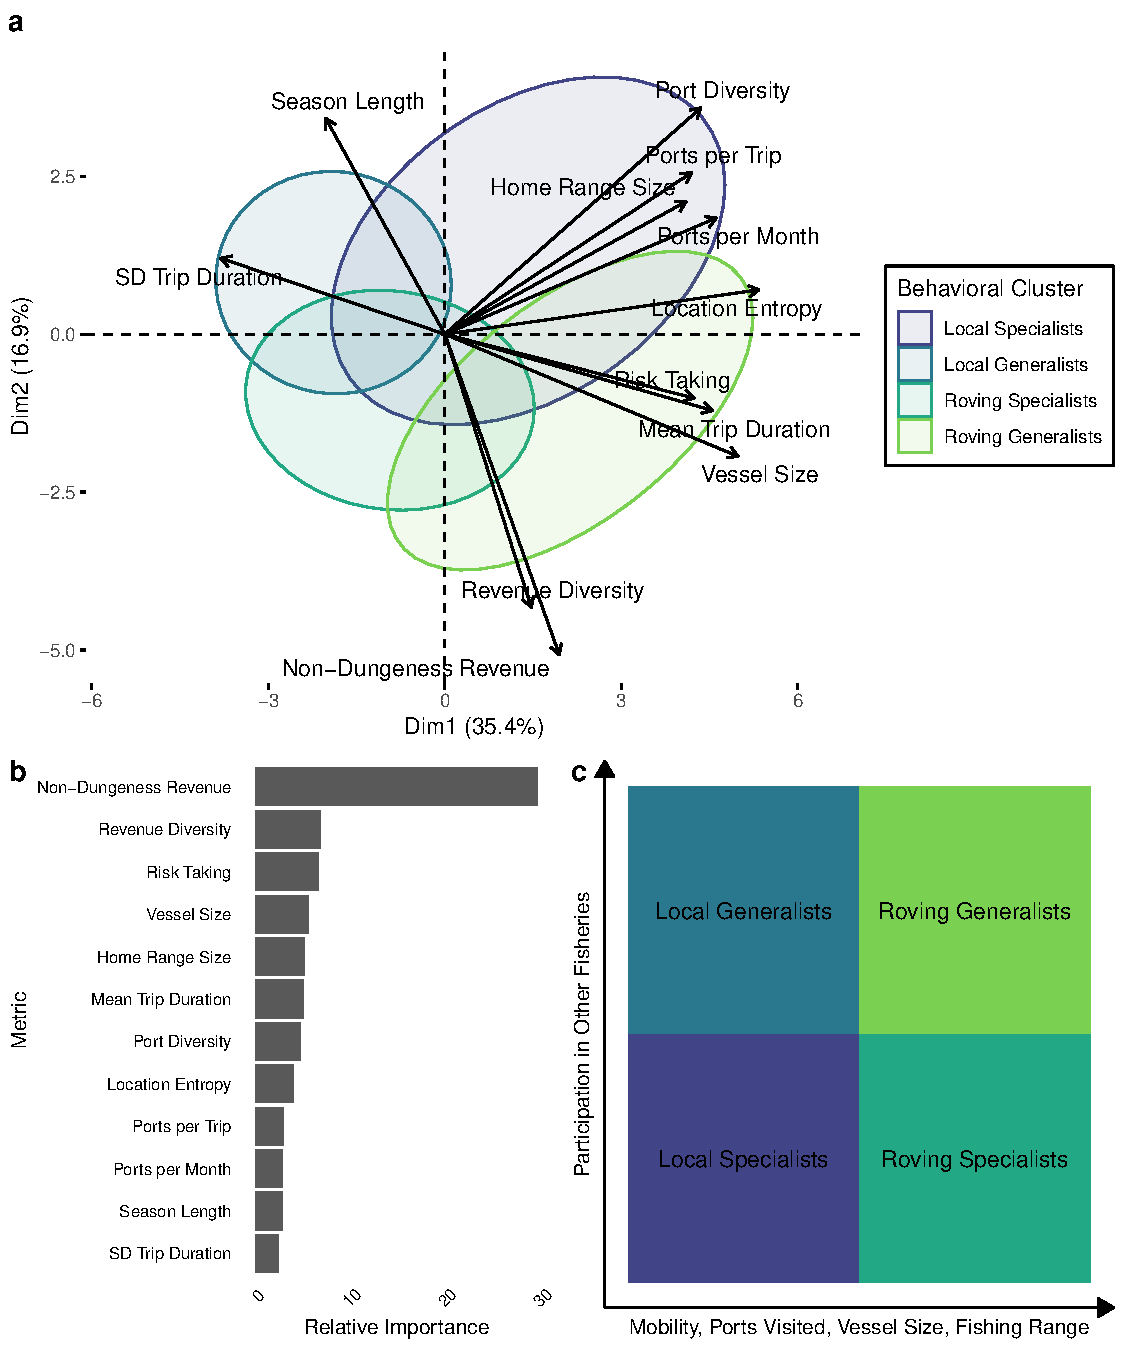
\includegraphics [width=\linewidth]{fig_pca_rf.pdf}
\caption{Data-driven formation of fishing behavioral groups. (a) Principal component analysis of vessel-seasons. Clusters of vessel-seasons, which determine behavioral groups, are enclosed by ellipses. Arrows represent the association between metrics in the cluster analysis relative to the placement of vessel-seasons. (b) Ranked importance of metrics used to classify vessel-seasons into behavioral groups, as determined by random forest analysis.(c) Conceptual visualization of the major axes defining behavioral groups.}
\label{fig:pca}
\end{figure}

\begin{figure}% [tbhp]
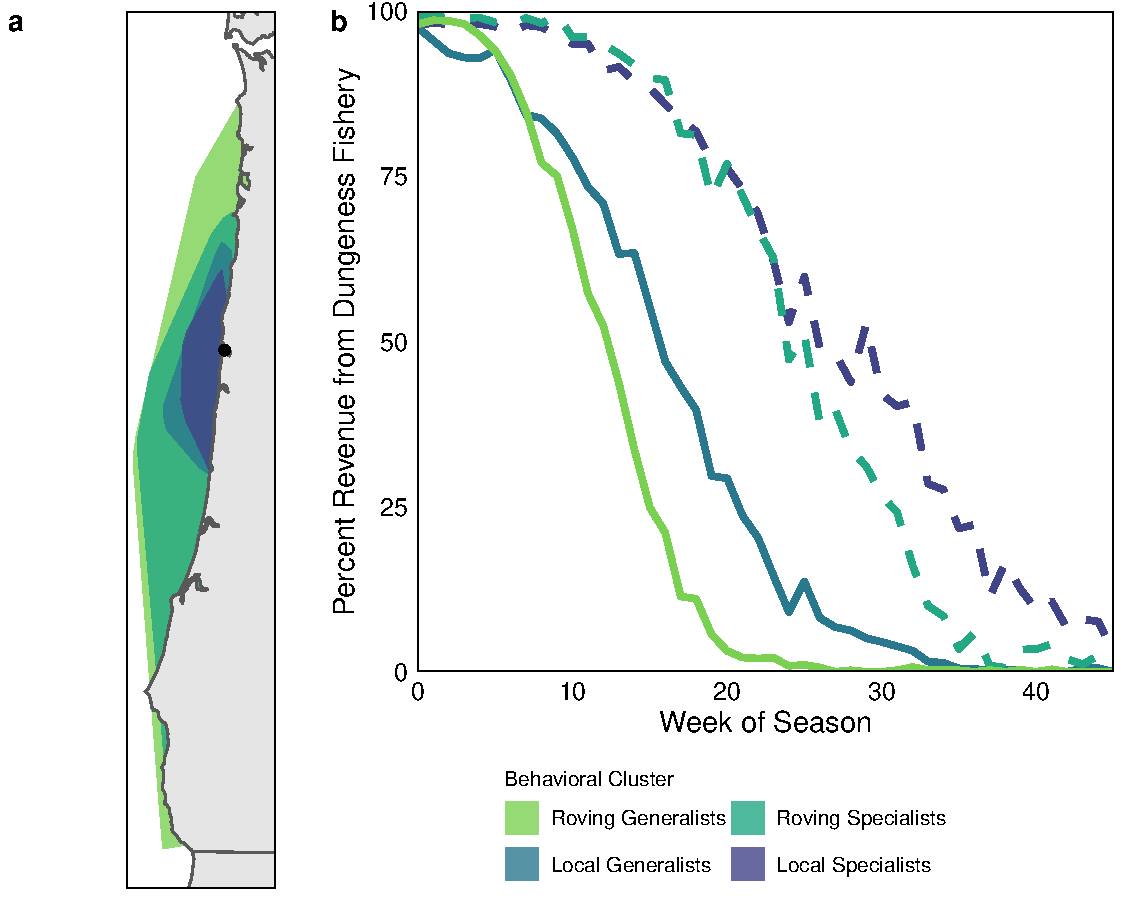
\includegraphics [width=\linewidth]{groups_mobility_flexibility.pdf}
\caption{Characteristic patterns in spatial mobility and fishery flexibility across behavioral groups in the west coast Dungeness crab fishery, exemplified by an Oregon port. (a) Fishing footprints of each behavioral group across all seasons for vessels originating from the Port of Newport, Oregon, USA. Shaded polygons are 95 percent convex hulls of all VMS locations for each group. (b) Fishery flexibility, displayed as the percent of Dungeness crab revenue relative to total weekly revenue (across all fisheries) for vessels in each behavioral group. Weekly revenues are averaged across crab seasons and across all vessels in each group. Generalist groups are represented with solid lines, while Specialist groups are represented with dashed lines.}
\label{fig:characteristics}
\end{figure}

\begin{figure}% [tbhp]
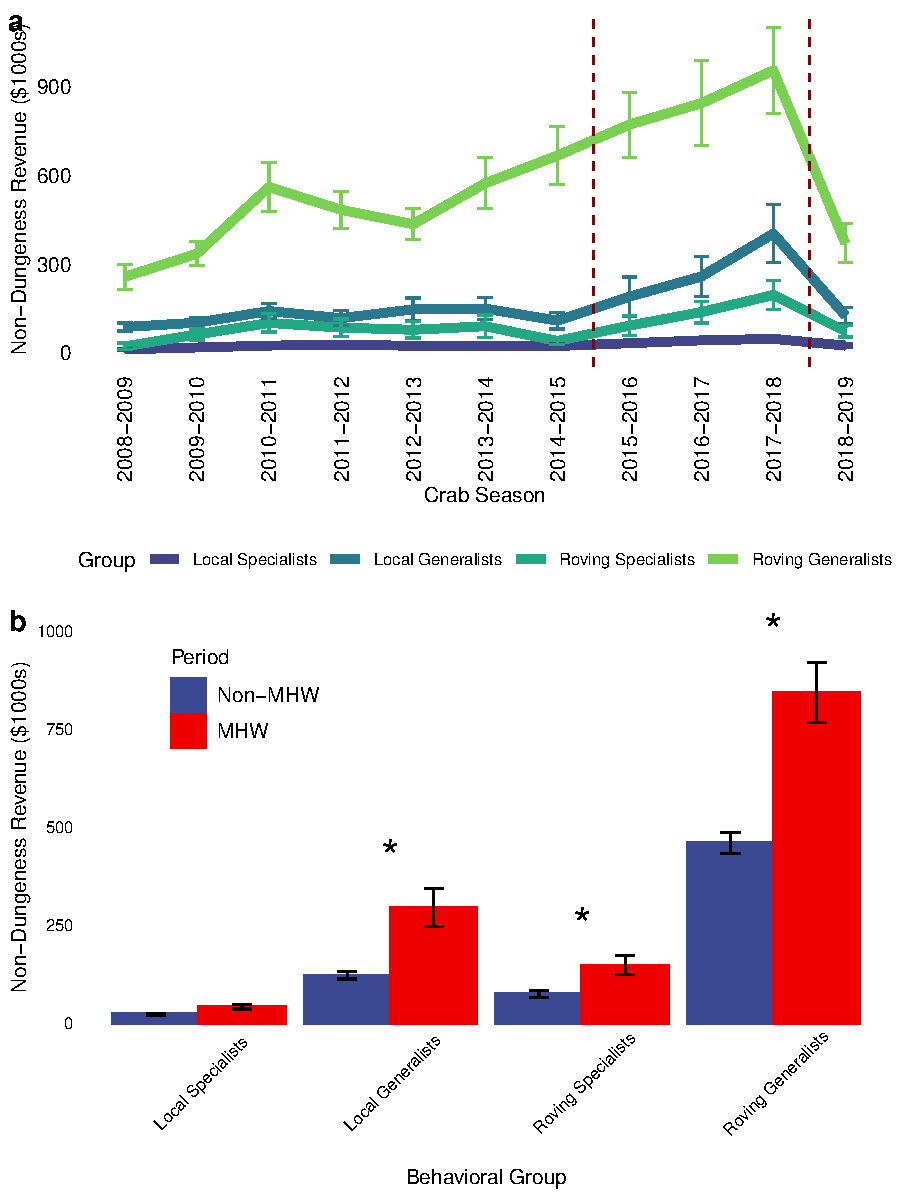
\includegraphics [width=\linewidth]{fig_nondcrb_revenue.pdf}
\caption{Non-Dungeness revenue for vessels in the analysis. (a) Seasonal mean revenue (+/- 2SE) for vessels in each behavioral group coming from all non-Dungeness fisheries combined. Vertical lines delineate the period of the marine heatwave (MHW). (b) Barplot of mean revenue (+/- 2SE) for vessels in each group during MHW and non-MHW seasons. Stars indicate groups with significantly different non-Dungeness revenue in MHW seasons.}
\label{fig:revenue}
\end{figure}

\begin{figure}% [tbhp]
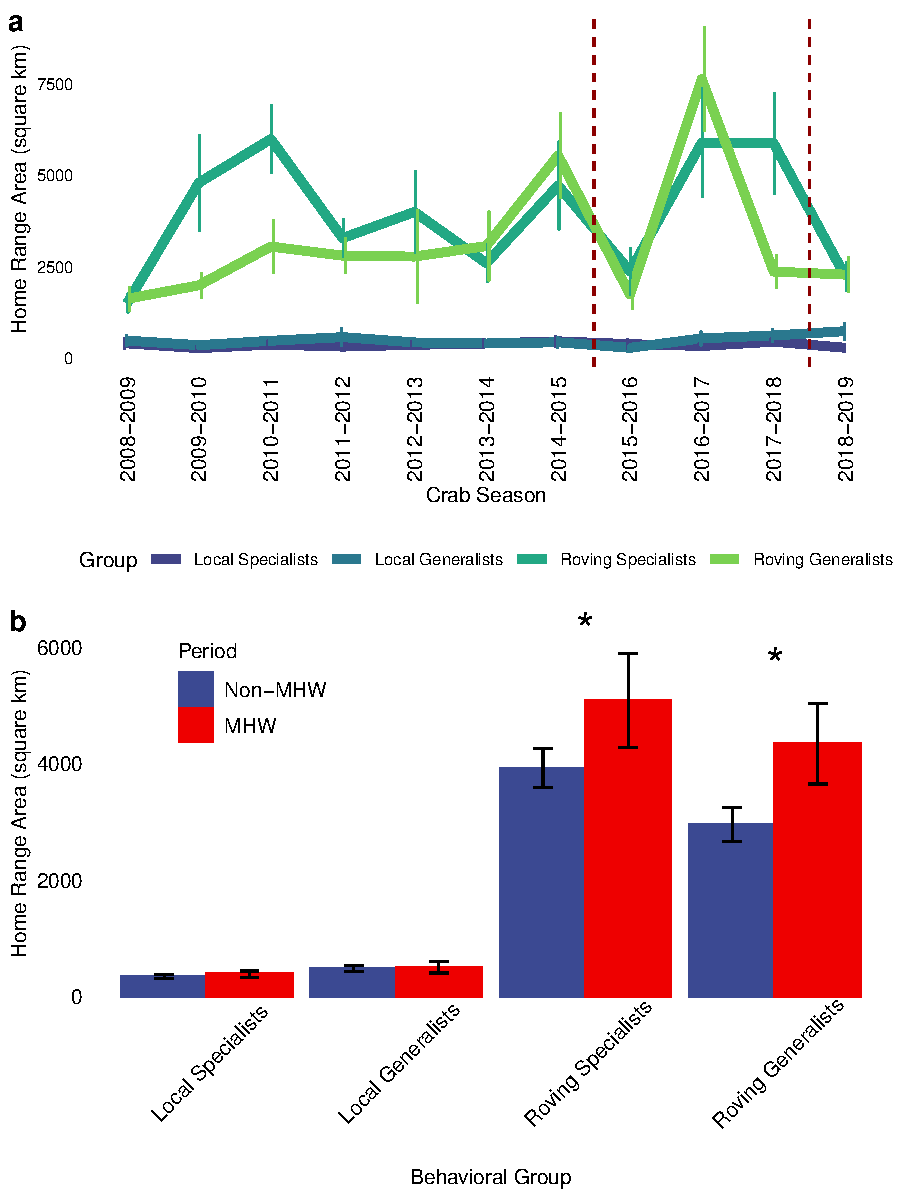
\includegraphics [width=\linewidth]{fig_homerange.pdf}
\caption{Home range (fishing area) size for vessels in the analysis. (a) Seasonal mean home range area in square kilometers (+/- 2SE) for vessels in each behavioral group. Vertical lines delineate the period of the MHW. (b) Barplot of mean home range area (+/- 2SE) for vessels in each group during MHW and non-MHW seasons. Stars indicate groups with significantly different home range size during MHW seasons.}
\label{fig:homerange}
\end{figure}

\begin{figure}% [tbhp]
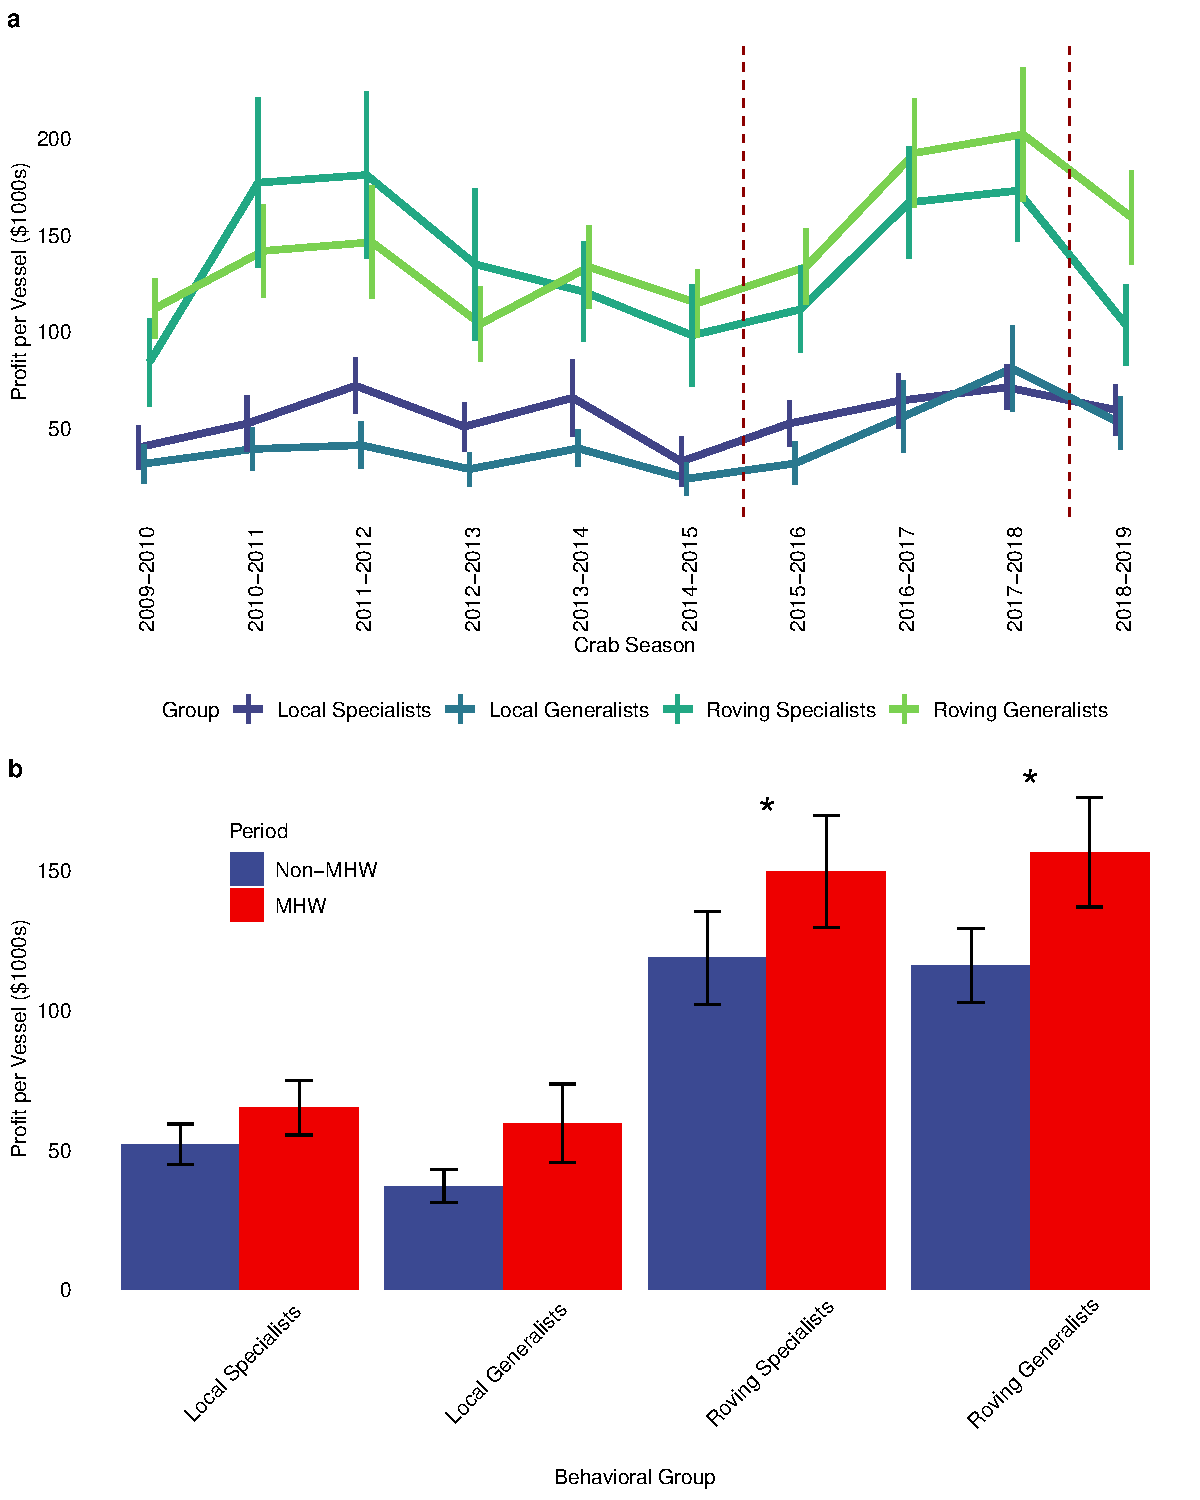
\includegraphics [width=\linewidth]{fig_profits.pdf}
\caption{Estimated profits by behavioral group. (a) Mean profit (+/- 2 SE) for vessels in each behavioral group over the full crab season. Vertical lines delineate the period of the marine heatwave. (b) Mean profit (+/- 2 SE) for each group in heatwave (MHW) versus non-MHW seasons. Stars indicate groups with significantly different estimated profits during MHW seasons.}
\label{fig:profits}
\end{figure}

\hypertarget{refs}{%
\section*{References}\label{refs}}
\addcontentsline{toc}{section}{References}

\hypertarget{refs}{}
\leavevmode\hypertarget{ref-Abatzoglou2019}{}%
Abatzoglou, J.T., Williams, A.P., Barbero, R., 2019. Global emergence of
anthropogenic climate change in fire weather indices. Geophysical
Research Letters 46, 326--336.
doi:\href{https://doi.org/10.1029/2018GL080959}{10.1029/2018GL080959}

\leavevmode\hypertarget{ref-Abrahms2018}{}%
Abrahms, B., Hazen, E.L., Bograd, S.J., Brashares, J.S., Robinson, P.W.,
Scales, K.L., Crocker, D.E., Costa, D.P., 2018. Climate mediates the
success of migration strategies in a marine predator. Ecology Letters
21, 63--71.
doi:\href{https://doi.org/10.1111/ele.12871}{10.1111/ele.12871}

\leavevmode\hypertarget{ref-Ager2011}{}%
Ager, A.A., Vaillant, N.M., Finney, M.A., 2011. Integrating fire
behavior models and geospatial analysis for wildland fire risk
assessment and fuel management planning. Journal of Combustion 2011.
doi:\href{https://doi.org/10.1155/2011/572452}{10.1155/2011/572452}

\leavevmode\hypertarget{ref-Allen1986}{}%
Allen, P.M., McGlade, J.M., 1986. Dynamics of discovery and
exploitation: The case of the scotian shelf groundfish fisheries.
Canadian Journal of Fisheries and Aquatic Sciences 43, 1187--1200.

\leavevmode\hypertarget{ref-Allison2001}{}%
Allison, E.H., Ellis, F., 2001. The livelihoods approach and management
of small-scale fisheries. Marine Policy 25, 377--388.

\leavevmode\hypertarget{ref-barnes2020social}{}%
Barnes, M.L., Wang, P., Cinner, J.E., Graham, N.A., Guerrero, A.M.,
Jasny, L., Lau, J., Sutcliffe, S.R., Zamborain-Mason, J., 2020. Social
determinants of adaptive and transformative responses to climate change.
Nature Climate Change 10, 823--828.

\leavevmode\hypertarget{ref-Beever2017}{}%
Beever, E.A., Hall, L.E., Varner, J., Loosen, A.E., Dunham, J.B., Gahl,
M.K., Smith, F.A., Lawler, J.J., 2017. Behavioral flexibility as a
mechanism for coping with climate change. Frontiers in Ecology and the
Environment 15, 299--308.
doi:\href{https://doi.org/10.1002/fee.1502}{10.1002/fee.1502}

\leavevmode\hypertarget{ref-Bellquist2021}{}%
Bellquist, L., Saccomanno, V., Semmens, B.X., Gleason, M., Wilson, J.,
2021. The rise in climate change-induced federal fishery disasters in
the united states. PeerJ 9.
doi:\href{https://doi.org/10.7717/peerj.11186}{10.7717/peerj.11186}

\leavevmode\hypertarget{ref-Bradley2019}{}%
Bradley, D., Merrifield, M., Miller, K.M., Lomonico, S., Wilson, J.R.,
Gleason, M.G., 2019. Opportunities to improve fisheries management
through innovative technology and advanced data systems. Fish and
Fisheries 20, 564--583.
doi:\href{https://doi.org/10.1111/faf.12361}{10.1111/faf.12361}

\leavevmode\hypertarget{ref-Branch2006}{}%
Branch, T.A., Hilborn, R., Haynie, A.C., Fay, G., Flynn, L., Griffiths,
J., Marshall, K.N., Randall, J.K., Scheuerell, J.M., Ward, E.J., Young,
M., 2006. Fleet dynamics and fishermen behavior: Lessons for fisheries
managers. Canadian Journal of Fisheries and Aquatic Sciences 63,
1647--1668.

\leavevmode\hypertarget{ref-Brodie2020}{}%
Brodie, J.F., Fragoso, J.M.V., 2020. Understanding the distribution of
bushmeat hunting effort across landscapes by testing hypotheses about
human foraging. Conservation Biology 0, 1--10.
doi:\href{https://doi.org/10.1111/cobi.13612}{10.1111/cobi.13612}

\leavevmode\hypertarget{ref-Burge2014}{}%
Burge, C.A., Eakin, C.M., Friedman, C.S., Froelich, B., Hershberger,
P.K., Hofmann, E.E., Petes, L.E., Prager, K.C., Weil, E., Willis, B.L.,
Ford, S.E., Harvell, C.D., 2014. Climate change influences on marine
infectious diseases: Implications for management and society. Annual
Review of Marine Science 6, 249--277.
doi:\href{https://doi.org/10.1146/annurev-marine-010213-135029}{10.1146/annurev-marine-010213-135029}

\leavevmode\hypertarget{ref-Cabral2018}{}%
Cabral, R.B., Mayorga, J., Clemence, M., Lynham, J., Koeshendrajana, S.,
Muawanah, U., Nugroho, D., Anna, Z., Ghofar, A., Zulbainarni, N.,
others, 2018. Rapid and lasting gains from solving illegal fishing.
Nature Ecology \& Evolution 2, 650--658.

\leavevmode\hypertarget{ref-Cavole2016}{}%
Cavole, L.M., Demko, A.M., Diner, R.E., Giddings, A., Koester, I.,
Pagniello, C.M., Paulsen, M.-L., Ramirez-Valdez, A., Schwenck, S.M.,
Yen, N.K., others, 2016. Biological impacts of the 2013--2015 warm-water
anomaly in the northeast pacific: Winners, losers, and the future.
Oceanography 29, 273--285.

\leavevmode\hypertarget{ref-nbclust2014}{}%
Charrad, M., Ghazzali, N., Boiteau, V., Niknafs, A., 2014. NbClust: An R
package for determining the relevant number of clusters in a data set.
Journal of Statistical Software 61, 1--36.

\leavevmode\hypertarget{ref-Cohen2007}{}%
Cohen, J.D., McClure, S.M., Yu, A.J., 2007. Should i stay or should i
go? How the human brain manages the trade-off between exploitation and
exploration. Philosophical Transactions of the Royal Society B:
Biological Sciences 362, 933--942.

\leavevmode\hypertarget{ref-Cook2018}{}%
Cook, B.I., Mankin, J.S., Anchukaitis, K.J., 2018. Climate change and
drought: From past to future. Current Climate Change Reports 4,
164--179.
doi:\href{https://doi.org/10.1007/s40641-018-0093-2}{10.1007/s40641-018-0093-2}

\leavevmode\hypertarget{ref-Dewees2004}{}%
Dewees, C.M., Sortais, K., Krachey, M.J., Hackett, S.C., Hankin, D.G.,
2004. Racing for crabs\ldots{} costs and management options evaluated in
dungeness crab fishery. California Agriculture 58, 186--189.
doi:\href{https://doi.org/10.3733/ca.v058n04p186}{10.3733/ca.v058n04p186}

\leavevmode\hypertarget{ref-Elmqvist2003a}{}%
Elmqvist, T., Folke, C., Nyström, M., Peterson, G., Bengtsson, J.,
Walker, B., Norberg, J., 2003. Response diversity, ecosystem change, and
resilience. Frontiers in Ecology and the Environment 1, 488--494.
doi:\href{https://doi.org/10.1890/1540-9295(2003)001\%5B0488:RDECAR\%5D2.0.CO;2}{10.1890/1540-9295(2003)001{[}0488:RDECAR{]}2.0.CO;2}

\leavevmode\hypertarget{ref-Feist2021}{}%
Feist, B.E., Samhouri, J.F., Forney, K.A., Saez, L.E., 2021. Footprints
of fixed-gear fisheries in relation to rising whale entanglements on the
u.s. West coast. Fisheries Management and Ecology 28, 283--294.
doi:\href{https://doi.org/10.1111/fme.12478}{10.1111/fme.12478}

\leavevmode\hypertarget{ref-Finkbeiner2015}{}%
Finkbeiner, E.M., 2015. The role of diversification in dynamic
small-scale fisheries: Lessons from baja california sur, mexico. Global
Environmental Change 32, 139--152.
doi:\href{https://doi.org/10.1016/j.gloenvcha.2015.03.009}{10.1016/j.gloenvcha.2015.03.009}

\leavevmode\hypertarget{ref-Fisher2021}{}%
Fisher, M.C., Moore, S.K., Jardine, S.L., Watson, J.R., Samhouri, J.F.,
2021. Climate shock effects and mediation in fisheries. Proceedings of
the National Academy of Sciences of the United States of America 118,
1--8.
doi:\href{https://doi.org/10.1073/pnas.2014379117}{10.1073/pnas.2014379117}

\leavevmode\hypertarget{ref-Frawley2020}{}%
Frawley, T.H., Muhling, B.A., Brodie, S., Fisher, M.C., Tommasi, D.,
Fol, G.L., Hazen, E.L., Stohs, S.S., Finkbeiner, E.M., Jacox, M.G.,
2020. Changes to the structure and function of an albacore fishery
reveal shifting social-ecological realities for pacific northwest
fishermen 1--18.
doi:\href{https://doi.org/10.1111/faf.12519}{10.1111/faf.12519}

\leavevmode\hypertarget{ref-Fryxell2017}{}%
Fryxell, J.M., Hilborn, R., Bieg, C., Turgeon, K., Caskenette, A.,
McCann, K.S., 2017. Supply and demand drive a critical transition to
dysfunctional fisheries. Proceedings of the National Academy of Sciences
of the United States of America 114, 12333--12337.
doi:\href{https://doi.org/10.1073/pnas.1705525114}{10.1073/pnas.1705525114}

\leavevmode\hypertarget{ref-Fuller2017}{}%
Fuller, E.C., Samhouri, J.F., Stoll, J.S., Levin, S.A., Watson, J.R.,
2017. Characterizing fisheries connectivity in marine social-ecological
systems. ICES Journal of Marine Science 74, 2087--2096.
doi:\href{https://doi.org/10.1093/icesjms/fsx128}{10.1093/icesjms/fsx128}

\leavevmode\hypertarget{ref-Fulton2011}{}%
Fulton, E.A., Smith, A.D.M., Smith, D.C., Putten, I.E.V., 2011. Human
behaviour: The key source of uncertainty in fisheries management. Fish
and Fisheries 12, 2--17.
doi:\href{https://doi.org/10.1111/j.1467-2979.2010.00371.x}{10.1111/j.1467-2979.2010.00371.x}

\leavevmode\hypertarget{ref-Gallagher2015}{}%
Gallagher, A.J., Hammerschlag, N., Cooke, S.J., Costa, D.P., Irschick,
D.J., 2015. Evolutionary theory as a tool for predicting extinction
risk. Trends in Ecology and Evolution 30, 61--65.
doi:\href{https://doi.org/10.1016/j.tree.2014.12.001}{10.1016/j.tree.2014.12.001}

\leavevmode\hypertarget{ref-Gladics2017}{}%
Gladics, A.J., Melvin, E.F., Suryan, R.M., Good, T.P., Jannot, J.E.,
Guy, T.J., 2017. Fishery-specific solutions to seabird bycatch in the
u.s. West coast sablefish fishery. Fisheries Research 196, 85--95.
doi:\href{https://doi.org/10.1016/j.fishres.2017.08.015}{10.1016/j.fishres.2017.08.015}

\leavevmode\hypertarget{ref-Gordon1954}{}%
Gordon, H.S., 1954. The economic theory of a common-property resource:
The fishery. The Journal of Political Economy 124--142.

\leavevmode\hypertarget{ref-Hamilton2019}{}%
Hamilton, S., Baker, G.B., 2019. Technical mitigation to reduce marine
mammal bycatch and entanglement in commercial fishing gear: Lessons
learnt and future directions. Reviews in Fish Biology and Fisheries 29,
223--247.
doi:\href{https://doi.org/10.1007/s11160-019-09550-6}{10.1007/s11160-019-09550-6}

\leavevmode\hypertarget{ref-Hankin2005}{}%
Hankin, D.G., Hackett, S.C., Dewees, C.M., 2005. California's dungeness
crab: Conserving the resource and increasing the net economic value of
the fishery. UC San Diego: California Sea Grant College Program.

\leavevmode\hypertarget{ref-Hartigan1979}{}%
Hartigan, J.A., Wong, M.A., 1979. Algorithm as 136: A k-means clustering
algorithm. Journal of the royal statistical society. series c (applied
statistics) 28, 100--108.

\leavevmode\hypertarget{ref-Hazen2018}{}%
Hazen, E.L., Scales, K.L., Maxwell, S.M., Briscoe, D.K., Welch, H.,
Bograd, S.J., Bailey, H., Benson, S.R., Eguchi, T., Dewar, H., others,
2018. A dynamic ocean management tool to reduce bycatch and support
sustainable fisheries. Science advances 4, eaar3001.

\leavevmode\hypertarget{ref-Hilborn1985}{}%
Hilborn, R., 1985. Fleet dynamics and individual variation: Why some
people catch more fish than others. Canadian Journal of Fisheries and
Aquatic Sciences 42, 2--13.
doi:\href{https://doi.org/10.1139/f85-001}{10.1139/f85-001}

\leavevmode\hypertarget{ref-Hinder2012}{}%
Hinder, S.L., Hays, G.C., Edwards, M., Roberts, E.C., Walne, A.W.,
Gravenor, M.B., 2012. Changes in marine dinoflagellate and diatom
abundance under climate change. Nature Climate Change 2, 271--275.
doi:\href{https://doi.org/10.1038/nclimate1388}{10.1038/nclimate1388}

\leavevmode\hypertarget{ref-Holland2020}{}%
Holland, D.S., Abbott, J.K., Norman, K.E., 2020. Fishing to live or
living to fish: Job satisfaction and identity of west coast fishermen.
Ambio 49, 628--639.
doi:\href{https://doi.org/10.1007/s13280-019-01206-w}{10.1007/s13280-019-01206-w}

\leavevmode\hypertarget{ref-Holland2017}{}%
Holland, D.S., Speir, C., Agar, J., Crosson, S., Depiper, G., Kasperski,
S., Kitts, A.W., Perruso, L., 2017. Impact of catch shares on
diversification of fishers' income and risk. Proceedings of the National
Academy of Sciences of the United States of America 114, 9302--9307.
doi:\href{https://doi.org/10.1073/pnas.1702382114}{10.1073/pnas.1702382114}

\leavevmode\hypertarget{ref-Jardine2020}{}%
Jardine, S.L., Fisher, M.C., Moore, S.K., Samhouri, J.F., 2020.
Inequality in the economic impacts from climate shocks in fisheries: The
case of harmful algal blooms. Ecological Economics 176, 106691.
doi:\href{https://doi.org/10.1016/j.ecolecon.2020.106691}{10.1016/j.ecolecon.2020.106691}

\leavevmode\hypertarget{ref-Joo2015}{}%
Joo, R., Salcedo, O., Gutierrez, M., Fablet, R., Bertrand, S., 2015.
Defining fishing spatial strategies from vms data: Insights from the
world's largest monospecific fishery. Fisheries Research 164, 223--230.
doi:\href{https://doi.org/10.1016/j.fishres.2014.12.004}{10.1016/j.fishres.2014.12.004}

\leavevmode\hypertarget{ref-Kasperski2013}{}%
Kasperski, S., Holland, D.S., 2013. Income diversification and risk for
fishermen. Proceedings of the National Academy of Sciences 110,
2076--2081.

\leavevmode\hypertarget{ref-Krofcheck2018}{}%
Krofcheck, D.J., Hurteau, M.D., Scheller, R.M., Loudermilk, E.L., 2018.
Prioritizing forest fuels treatments based on the probability of
high-severity fire restores adaptive capacity in sierran forests. Global
Change Biology 24, 729--737.
doi:\href{https://doi.org/10.1111/gcb.13913}{10.1111/gcb.13913}

\leavevmode\hypertarget{ref-Leslie2015}{}%
Leslie, H.M., Basurto, X., Nenadovic, M., Sievanen, L., Cavanaugh, K.C.,
Cota-Nieto, J.J., Erisman, B.E., Finkbeiner, E., Hinojosa-Arango, G.,
Moreno-Báez, M., Nagavarapu, S., Reddy, S.M.W., Sánchez-Rodríguez, A.,
Siegel, K., Ulibarria-Valenzuela, J.J., Weaver, A.H., Aburto-Oropeza,
O., 2015. Operationalizing the social-ecological systems framework to
assess sustainability. Proceedings of the National Academy of Sciences
of the United States of America 112, 5979--5984.
doi:\href{https://doi.org/10.1073/pnas.1414640112}{10.1073/pnas.1414640112}

\leavevmode\hypertarget{ref-Wiener2003}{}%
Liaw, A., Wiener, M., 2002. Classification and regression by
randomForest. R News 3, 18--22.

\leavevmode\hypertarget{ref-Lubchenco2016}{}%
Lubchenco, J., Cerny-Chipman, E.B., Reimer, J.N., Levin, S.A., 2016. The
right incentives enable ocean sustainability successes and provide hope
for the future. Proceedings of the National Academy of Sciences of the
United States of America 113, 14507--14514.
doi:\href{https://doi.org/10.1073/pnas.1604982113}{10.1073/pnas.1604982113}

\leavevmode\hypertarget{ref-Mancilla2020}{}%
Mancilla Garcia, M., Hertz, T., Schluter, M., Preiser, R., Woermann, M.,
2020. Adopting process-relational perspectives to tackle the challenges
of social-ecological systems research. Ecology and Society 25.

\leavevmode\hypertarget{ref-Mao2020}{}%
Mao, J., Jardine, S.L., 2020. Market impacts of a toxic algae event: The
case of california dungeness crab. Marine Resource Economics 35, 1--20.
doi:\href{https://doi.org/10.1086/707643}{10.1086/707643}

\leavevmode\hypertarget{ref-Maxwell2015}{}%
Maxwell, S.M., Hazen, E.L., Lewison, R.L., Dunn, D.C., Bailey, H.,
Bograd, S.J., Briscoe, D.K., Fossette, S., Hobday, A.J., Bennett, M.,
Benson, S., Caldwell, M.R., Costa, D.P., Dewar, H., Eguchi, T., Hazen,
L., Kohin, S., Sippel, T., Crowder, L.B., 2015. Dynamic ocean
management: Defining and conceptualizing real-time management of the
ocean. Marine Policy 58, 42--50.
doi:\href{https://doi.org/10.1016/j.marpol.2015.03.014}{10.1016/j.marpol.2015.03.014}

\leavevmode\hypertarget{ref-McCabe2016}{}%
McCabe, R.M., Hickey, B.M., Kudela, R.M., Lefebvre, K.A., Adams, N.G.,
Bill, B.D., Gulland, F.M.D., Thomson, R.E., Cochlan, W.P., Trainer,
V.L., 2016. An unprecedented coastwide toxic algal bloom linked to
anomalous ocean conditions. Geophysical Research Letters 43, 10,
366--10, 376.
doi:\href{https://doi.org/10.1002/2016GL070023}{10.1002/2016GL070023}

\leavevmode\hypertarget{ref-Mcginnis2014}{}%
Mcginnis, M.D., Ostrom, E., 2014. Social-ecological system framework :
Initial changes and continuing challenges. Ecology and Society 19.

\leavevmode\hypertarget{ref-Mendo2019}{}%
Mendo, T., Smout, S., Photopoulou, T., James, M., 2019. Identifying
fishing grounds from vessel tracks: Model-based inference for small
scale fisheries. Royal Society Open Science 6.
doi:\href{https://doi.org/10.1098/rsos.191161}{10.1098/rsos.191161}

\leavevmode\hypertarget{ref-Moore2020harmful}{}%
Moore, K.M., Allison, E.H., Dreyer, S.J., Ekstrom, J.A., Jardine, S.L.,
Klinger, T., Moore, S.K., Norman, K.C., 2020a. Harmful algal blooms:
Identifying effective adaptive actions used in fishery-dependent
communities in response to a protracted event. Frontiers in Marine
Science 6, 803.

\leavevmode\hypertarget{ref-Moore2020}{}%
Moore, S.K., Dreyer, S.J., Ekstrom, J.A., Moore, K., Norman, K.,
Klinger, T., Allison, E.H., Jardine, S.L., 2020b. Harmful algal blooms
and coastal communities: Socioeconomic impacts and actions taken to cope
with the 2015 u.s. West coast domoic acid event. Harmful Algae 96,
101799.
doi:\href{https://doi.org/10.1016/j.hal.2020.101799}{10.1016/j.hal.2020.101799}

\leavevmode\hypertarget{ref-OFarrell2019}{}%
O'Farrell, S., Chollett, I., Sanchirico, J.N., Perruso, L., 2019a.
Classifying fishing behavioral diversity using high-frequency movement
data. Proceedings of the National Academy of Sciences 116, 16811--16816.
doi:\href{https://doi.org/10.1073/pnas.1906766116}{10.1073/pnas.1906766116}

\leavevmode\hypertarget{ref-OFarrell2019a}{}%
O'Farrell, S., Sanchirico, J.N., Spiegel, O., Depalle, M., Haynie, A.C.,
Murawski, S.A., Perruso, L., Strelcheck, A., 2019b. Disturbance modifies
payoffs in the explore-exploit trade-off. Nature Communications 10,
1--9.
doi:\href{https://doi.org/10.1038/s41467-019-11106-y}{10.1038/s41467-019-11106-y}

\leavevmode\hypertarget{ref-Oken2021}{}%
Oken, K.L., Holland, D.S., Andr´, A., Punt, A.E., 2021. The effects of
population synchrony, life history, and access constraints on benefits
from fishing portfolios.

\leavevmode\hypertarget{ref-Oliver2018}{}%
Oliver, E.C.J., Donat, M.G., Burrows, M.T., Moore, P.J., Smale, D.A.,
Alexander, L.V., Benthuysen, J.A., Feng, M., Gupta, A.S., Hobday, A.J.,
Holbrook, N.J., Perkins-Kirkpatrick, S.E., Scannell, H.A., Straub, S.C.,
Wernberg, T., 2018. Longer and more frequent marine heatwaves over the
past century. Nature Communications 9, 1--12.
doi:\href{https://doi.org/10.1038/s41467-018-03732-9}{10.1038/s41467-018-03732-9}

\leavevmode\hypertarget{ref-Papaioannou2021}{}%
Papaioannou, E.A., Selden, R.L., Olson, J., McCay, B.J., Pinsky, M.L.,
Martin, K.S., 2021. Not all those who wander are lost -- responses of
fishers' communities to shifts in the distribution and abundance of
fish. Frontiers in Marine Science 8.
doi:\href{https://doi.org/10.3389/fmars.2021.669094}{10.3389/fmars.2021.669094}

\leavevmode\hypertarget{ref-Pellowe2019}{}%
Pellowe, K.E., Leslie, H.M., 2019. Heterogeneity among clam harvesters
in northwest mexico shapes individual adaptive capacity. Ecology and
Society 24.
doi:\href{https://doi.org/10.5751/ES-11297-240425}{10.5751/ES-11297-240425}

\leavevmode\hypertarget{ref-Pfeiffer2016}{}%
Pfeiffer, L., Gratz, T., 2016. The effect of rights-based fisheries
management on risk taking and fishing safety. Proceedings of the
National Academy of Sciences of the United States of America 113,
2615--2620.
doi:\href{https://doi.org/10.1073/pnas.1509456113}{10.1073/pnas.1509456113}

\leavevmode\hypertarget{ref-Pollnac2008}{}%
Pollnac, R.B., Poggie, J.J., 2008. Happiness, well-being and
psychocultural adaptation to the stresses associated with marine
fishing. Human Ecology Review 194--200.

\leavevmode\hypertarget{ref-Pollnac1998}{}%
Pollnac, R., Poggie, J., Cabral, S., 1998. Thresholds of danger:
Perceived risk in a new england fishery. Human organization 57, 53--59.

\leavevmode\hypertarget{ref-Rasmuson2013}{}%
Rasmuson, L.K., 2013. The biology, ecology and fishery of the dungeness
crab, cancer magister, 1st ed, Advances in Marine Biology. Elsevier Ltd.
doi:\href{https://doi.org/10.1016/B978-0-12-410498-3.00003-3}{10.1016/B978-0-12-410498-3.00003-3}

\leavevmode\hypertarget{ref-RCoreTeam2021}{}%
R Core Team, 2021. R: A language and environment for statistical
computing. R Foundation for Statistical Computing, Vienna, Austria.

\leavevmode\hypertarget{ref-Renner2015}{}%
Renner, M., Kuletz, K.J., 2015. A spatial-seasonal analysis of the
oiling risk from shipping traffic to seabirds in the aleutian
archipelago. Marine Pollution Bulletin 101, 127--136.
doi:\href{https://doi.org/10.1016/j.marpolbul.2015.11.007}{10.1016/j.marpolbul.2015.11.007}

\leavevmode\hypertarget{ref-Richerson2020}{}%
Richerson, K., Punt, A.E., Holland, D.S., 2020. Nearly a half century of
high but sustainable exploitation in the dungeness crab (cancer
magister) fishery. Fisheries Research 226, 105528.
doi:\href{https://doi.org/10.1016/j.fishres.2020.105528}{10.1016/j.fishres.2020.105528}

\leavevmode\hypertarget{ref-Ritzman2018}{}%
Ritzman, J., Brodbeck, A., Brostrom, S., McGrew, S., Dreyer, S.,
Klinger, T., Moore, S.K., 2018. Economic and sociocultural impacts of
fisheries closures in two fishing-dependent communities following the
massive 2015 u.s. West coast harmful algal bloom. Harmful Algae 80,
35--45.
doi:\href{https://doi.org/10.1016/j.hal.2018.09.002}{10.1016/j.hal.2018.09.002}

\leavevmode\hypertarget{ref-Russell2018}{}%
Russell, S.M., Oostenburg, M.V., Vizek, A., 2018. Adapting to catch
shares: Perspectives of west coast groundfish trawl participants.
Coastal Management 46, 603--620.
doi:\href{https://doi.org/10.1080/08920753.2018.1522491}{10.1080/08920753.2018.1522491}

\leavevmode\hypertarget{ref-Salas2004}{}%
Salas, S., Gaertner, D., 2004. The behavioural dynamics of fishers:
Management implications. Fish and Fisheries 5, 153--167.
doi:\href{https://doi.org/10.1111/j.1467-2979.2004.00146.x}{10.1111/j.1467-2979.2004.00146.x}

\leavevmode\hypertarget{ref-Samhouri2021}{}%
Samhouri, J.F., Feist, B.E., Fisher, M.C., Liu, O., Woodman, S.M.,
Abrahms, B., Forney, K.A., Hazen, E.L., Lawson, D., Redfern, J., others,
2021. Marine heatwave challenges solutions to human--wildlife conflict.
Proceedings of the Royal Society B 288, 20211607.

\leavevmode\hypertarget{ref-Santora2020}{}%
Santora, J.A., Mantua, N.J., Schroeder, I.D., Field, J.C., Hazen, E.L.,
Bograd, S.J., Sydeman, W.J., Wells, B.K., Calambokidis, J., Saez, L.,
Lawson, D., Forney, K.A., 2020. Habitat compression and ecosystem shifts
as potential links between marine heatwave and record whale
entanglements. Nature Communications 2020 11:1 11, 1--12.
doi:\href{https://doi.org/10.1038/s41467-019-14215-w}{10.1038/s41467-019-14215-w}

\leavevmode\hypertarget{ref-Scholes2013}{}%
Scholes, R.J., Reyers, B., Biggs, R., Spierenburg, M., Duriappah, A.,
2013. Multi-scale and cross-scale assessments of social--ecological
systems and their ecosystem services. Current Opinion in Environmental
Sustainability 5, 16--25.

\leavevmode\hypertarget{ref-Smale2019}{}%
Smale, D.A., Wernberg, T., Oliver, E.C.J., Thomsen, M., Harvey, B.P.,
Straub, S.C., Burrows, M.T., Alexander, L.V., Benthuysen, J.A., Donat,
M.G., Feng, M., Hobday, A.J., Holbrook, N.J., Perkins-Kirkpatrick, S.E.,
Scannell, H.A., Gupta, A.S., Payne, B.L., Moore, P.J., 2019. Marine
heatwaves threaten global biodiversity and the provision of ecosystem
services. Nature Climate Change 9, 306--312.
doi:\href{https://doi.org/10.1038/s41558-019-0412-1}{10.1038/s41558-019-0412-1}

\leavevmode\hypertarget{ref-Smith1986}{}%
Smith, C.L., McKelvey, R., 1986. Specialist and generalist: Roles for
coping with variability. North American Journal of Fisheries Management
6, 88--99.
doi:\href{https://doi.org/10.1577/1548-8659(1986)6\%3C88:sag\%3E2.0.co;2}{10.1577/1548-8659(1986)6\textless88:sag\textgreater2.0.co;2}

\leavevmode\hypertarget{ref-Suryan2021}{}%
Suryan, R.M., Arimitsu, M.L., Coletti, H.A., Hopcroft, R.R., Lindeberg,
M.R., Barbeaux, S.J., Batten, S.D., Burt, W.J., Bishop, M.A., Bodkin,
J.L., Brenner, R., Campbell, R.W., Cushing, D.A., Danielson, S.L., Dorn,
M.W., Drummond, B., Esler, D., Gelatt, T., Hanselman, D.H., Hatch, S.A.,
Haught, S., Holderied, K., Iken, K., Irons, D.B., Kettle, A.B., Kimmel,
D.G., Konar, B., Kuletz, K.J., Laurel, B.J., Maniscalco, J.M., Matkin,
C., McKinstry, C.A.E., Monson, D.H., Moran, J.R., Olsen, D., Palsson,
W.A., Pegau, W.S., Piatt, J.F., Rogers, L.A., Rojek, N.A., Schaefer, A.,
Spies, I.B., Straley, J.M., Strom, S.L., Sweeney, K.L., Szymkowiak, M.,
Weitzman, B.P., Yasumiishi, E.M., Zador, S.G., 2021. Ecosystem response
persists after a prolonged marine heatwave. Scientific Reports 11,
1--17.
doi:\href{https://doi.org/10.1038/s41598-021-83818-5}{10.1038/s41598-021-83818-5}

\leavevmode\hypertarget{ref-Townhill2018}{}%
Townhill, B.L., Tinker, J., Jones, M., Pitois, S., Creach, V., Simpson,
S.D., Dye, S., Bear, E., Pinnegar, J.K., 2018. Harmful algal blooms and
climate change: Exploring future distribution changes. ICES Journal of
Marine Science 75, 1882--1893.
doi:\href{https://doi.org/10.1093/icesjms/fsy113}{10.1093/icesjms/fsy113}

\leavevmode\hypertarget{ref-VanLoon2016}{}%
Van Loon, A.F., Gleeson, T., Clark, J., Dijk, A.I.J.V., Stahl, K.,
Hannaford, J., Baldassarre, G.D., Teuling, A.J., Tallaksen, L.M.,
Uijlenhoet, R., Hannah, D.M., Sheffield, J., Svoboda, M., Verbeiren, B.,
Wagener, T., Rangecroft, S., Wanders, N., Lanen, H.A.J.V., 2016. Drought
in the anthropocene. Nature Geoscience 9, 89--91.
doi:\href{https://doi.org/10.1038/ngeo2646}{10.1038/ngeo2646}

\leavevmode\hypertarget{ref-VonBiela2019}{}%
von Biela, V., Arimitsu, M.L., Piatt, J.F., Heflin, B.M., Schoen, S.,
2019. Extreme reduction in condition of a key forage fish during the
pacific marine heatwave of 2014--2016. Marine Ecology Progress Series
613, 171--182.

\leavevmode\hypertarget{ref-Watson2018}{}%
Watson, J.R., Fuller, E.C., Castruccio, F.S., Samhouri, J.F., 2018.
Fishermen follow fine-scale physical ocean features for finance.
Frontiers in Marine Science 5, 46.

\leavevmode\hypertarget{ref-Watson2016}{}%
Watson, J.T., Haynie, A.C., 2016. Using vessel monitoring system data to
identify and characterize trips made by fishing vessels in the united
states north pacific. PLoS ONE 11, 1--20.
doi:\href{https://doi.org/10.1371/journal.pone.0165173}{10.1371/journal.pone.0165173}

\leavevmode\hypertarget{ref-Wilson2018}{}%
Wilson, J.R., Lomonico, S., Bradley, D., Sievanen, L., Dempsey, T.,
Bell, M., McAfee, S., Costello, C., Szuwalski, C., McGonigal, H.,
Fitzgerald, S., Gleason, M., 2018. Adaptive comanagement to achieve
climate-ready fisheries. Conservation Letters 11, 1--7.
doi:\href{https://doi.org/10.1111/conl.12452}{10.1111/conl.12452}

\leavevmode\hypertarget{ref-Young2019}{}%
Young, T., Fuller, E.C., Provost, M.M., Coleman, K.E., Martin, K.S.,
McCay, B.J., Pinsky, M.L., 2019. Adaptation strategies of coastal
fishing communities as species shift poleward. ICES Journal of Marine
Science 76, 93--103.
doi:\href{https://doi.org/10.1093/icesjms/fsy140}{10.1093/icesjms/fsy140}


\end{document}

